\documentclass[11pt,a4paper]{article}

% ---- Packages ----
\usepackage[utf8]{inputenc}
\usepackage[T1]{fontenc}
\usepackage{mathpazo}           % Palatino font (matches MDPI)
\usepackage{amsmath,amssymb}
\usepackage{graphicx}
\usepackage{booktabs}
\usepackage{longtable}
\usepackage{tabularx}
\usepackage{float}
\usepackage{geometry}
\usepackage{setspace}
\usepackage{xcolor}
\usepackage[
  colorlinks=true,
  linkcolor={blue!70!black},
  citecolor={red!60!black},
  urlcolor={teal!80!black}
]{hyperref}
\usepackage{cleveref}
\usepackage{caption}
\usepackage{pdflscape}          % landscape pages for wide tables

% ---- Page layout ----
\geometry{margin=2.5cm}
\onehalfspacing
\setlength{\parindent}{0pt}
\setlength{\parskip}{6pt plus 2pt minus 1pt}

% ---- Font sizes ----
% Smaller captions for figures and tables
\captionsetup{font=small, labelfont=bf}
% Equation numbers on the right (default in article class)

% ---- Pandoc compat ----
\providecommand{\tightlist}{\setlength{\itemsep}{0pt}\setlength{\parskip}{0pt}}

% ---- Line numbers for review ----
\usepackage{lineno}
\linenumbers

% ---- Section font sizes (scaled for 11pt body) ----
\usepackage{titlesec}
\titleformat{\section}{\large\bfseries}{\thesection}{1em}{}
\titleformat{\subsection}{\normalsize\bfseries}{\thesubsection}{1em}{}
\titleformat{\subsubsection}{\normalsize\itshape}{\thesubsubsection}{1em}{}
\titleformat{\paragraph}[runin]{\normalsize\bfseries}{\theparagraph}{1em}{}[.]

% ============================================================
\title{\Large A Modular Framework for Enhancing Satellite-Derived Daily Precipitation: Adjusting Values, Aligning Distributions, and Preserving Extremes}


\author{\normalsize
Benny Istanto\textsuperscript{1,*} \and
Rizaldi Boer\textsuperscript{2,3} \and
I Putu Santikayasa\textsuperscript{2,4}
}

\date{\small
\textsuperscript{1} Applied Climatology Study Program, Department of Geophysics and Meteorology,\\
Bogor Agricultural University, Bogor 16680, Indonesia\\[2pt]
\textsuperscript{2} Department of Geophysics and Meteorology, Bogor Agricultural University, Bogor 16680, Indonesia\\[2pt]
\textsuperscript{3} International Research Institute for Environment and Climate Change,\\
Bogor Agricultural University, Bogor 16680, Indonesia\\[2pt]
\textsuperscript{4} Center for Climate Risk and Opportunity Management in South East Asia and Pacific,\\
Bogor Agricultural University, Bogor 16680, Indonesia\\[6pt]
* Correspondence: bennyistanto@gmail.com
}

\begin{document}
\maketitle

\begin{abstract}
Accurate daily precipitation estimates are essential for hydrological modeling, climate risk assessment, and disaster preparedness. Satellite-based precipitation products such as the Integrated Multi-satellitE Retrievals for Global Precipitation Measurement (IMERG) provide global coverage but exhibit systematic biases in daily accumulations, particularly in representing extreme precipitation events. This study presents a hybrid bias correction framework (LSEQM+DL) for daily satellite precipitation that sequentially integrates Linear Scaling (LS) for mean bias removal, Empirical Quantile Mapping (EQM) with Generalized Pareto Distribution (GPD) tail adjustment for distributional alignment, and a Convolutional Neural Network (CNN) refinement that selectively targets extreme precipitation pixels. A station density confidence mask modulates the deep learning influence based on gauge network density, so that the CNN refinement is strongest where the reference dataset (CPC Unified Gauge-Based Analysis of Daily Precipitation, CPC-UNI) is best constrained by observations. Applied to daily IMERG Late Run precipitation over Indonesia (2001--2025) and evaluated against CPC-UNI and 171 independent station observations from Indonesia's Meteorological, Climatological, and Geophysical Agency (BMKG), the framework is assessed through three evaluation pillars aligned with its design objectives: adjusting values, aligning distributions, and preserving extremes. At independent BMKG station locations, the hybrid correction brings the standard deviation ratio from 0.71 (LS) to 1.00 (LSEQM+DL, toward unity), the relative bias from $-$11.4\% to $-$0.6\%, and the 99th-percentile ratio from 0.71 to 1.01, indicating convergence of the corrected distribution toward the observed precipitation statistics. The wet-day frequency ratio improves from 1.21 (LS) to 0.95 (LSEQM+DL), reducing a 21\% overestimation of wet-day occurrence to within 5\% of observed. These improvements come at a known cost: event detection (POD) decreases from 0.78 to 0.65, reflecting the trade-off inherent to distributional correction methods that adjust marginal statistics without modifying temporal sequencing. Pixel-level temporal accuracy metrics (correlation, root mean square error, Nash-Sutcliffe efficiency) remain largely unchanged, confirming that the framework improves statistical properties rather than day-to-day prediction skill. The World Meteorological Organization (WMO) multi-threshold verification at station locations shows maintained detection skill at rainfall thresholds up to 100 mm/day. The framework relies on globally available satellite and gauge-analysis datasets, and its station-density-aware design degrades gracefully where gauge support is weak. Transfer to other tropical and subtropical regions is supported in principle by this property, with regional recalibration of the GPD threshold, blending weight, and saturation count expected.

\noindent\textbf{Keywords:} Bias Correction, Satellite Precipitation, IMERG, Daily Precipitation, Extreme Events, Deep Learning, Quantile Mapping, Generalized Pareto Distribution, Quality Assessment, Indonesia
\end{abstract}

\newpage


\section{Introduction}\label{introduction}

Accurate and timely precipitation estimates are critical for a wide
range of scientific and societal applications, including flood
forecasting, drought monitoring, hydrological modeling, and climate risk
assessments. Satellite-derived precipitation products, such as those
from the Global Precipitation Measurement (GPM) mission \cite{ref1,ref2}, have
greatly expanded the global coverage of precipitation observations,
especially over regions with sparse ground station networks. However,
despite their transformative role, satellite-based estimates often
suffer from systematic biases, spatial inconsistencies, and challenges
in capturing the full spectrum of precipitation variability \cite{ref3},
particularly for extreme rainfall events. These limitations reduce the
reliability of satellite data for operational and scientific
applications that depend on an accurate depiction of both mean
conditions and high-impact extremes.

A wide range of bias correction techniques has been developed to address
these challenges. Traditional statistical methods, such as Linear
Scaling (LS), effectively correct mean biases by adjusting the overall
magnitude of satellite estimates to align with ground-based observations
\cite{ref4}. Empirical Quantile Mapping (EQM) extends this correction by
aligning the entire distribution of satellite precipitation with the
reference distribution, adjusting not only the mean but also
higher-order statistical moments \cite{ref5,ref6}. More recently, methods such
as Generalized Pareto Distribution (GPD) fitting have been introduced to
specifically address biases in the tails of precipitation distributions,
aiming to better preserve extreme events \cite{ref7}. In parallel, advances
in machine learning (ML) and deep learning (DL) have opened new
possibilities for bias correction, enabling more flexible and nonlinear
mappings between satellite and reference data \cite{ref8}. Convolutional
Neural Networks (CNNs) provide powerful capabilities for modeling
complex spatial patterns that traditional statistical methods may
overlook \cite{ref9,ref10}.

Despite these advances, critical gaps remain. Traditional bias correction techniques often underperform in preserving the frequency and magnitude of extreme precipitation events \cite{ref8,ref11}, while many machine learning approaches lack integration with physically interpretable statistical corrections, risking overfitting or reduced transparency \cite{ref12}. There remains a need for a hybrid approach that simultaneously addresses mean biases, distributional alignment, and extreme event preservation within a single, modular pipeline.

In this study, we propose a hybrid bias correction framework that
sequentially integrates Linear Scaling, Empirical Quantile Mapping with
gamma-based distribution fitting and GPD tail adjustment, and a Deep
Learning refinement step using Convolutional Neural Networks. The
framework is designed to improve daily satellite precipitation estimates
by systematically adjusting mean values, aligning distributions, and
preserving extremes. Using globally available datasets -- the Integrated
Multi-satellitE Retrievals for GPM (IMERG) Late Run (IMERG-L) satellite
precipitation \cite{ref2} and the CPC Global Unified Gauge-Based Analysis of
Daily Precipitation (CPC-UNI) gridded station observations \cite{ref13} --
the methodology is demonstrated over the Indonesian archipelago,
selected for its vulnerability to extreme rainfall and complex
topographic and climatic conditions. Correction quality is evaluated
through 31 verification metrics organized into a composite Continuous
Quality Index (CQI), providing a structured assessment across basic
statistical, distributional, and temporal dimensions \cite{ref14,ref15}.

To address the spatial heterogeneity inherent in gauge-based reference
datasets, the framework incorporates a station density confidence mask
that modulates the influence of the deep learning component based on
gauge network density. In regions where the CPC-UNI reference is
supported by dense station coverage, the CNN refinement is applied with
greater confidence. In station-sparse regions, where the reference
dataset relies on interpolation and may not accurately capture local
precipitation characteristics, the framework reverts toward purely
statistical corrections. This design provides a systematic approach for
managing reference dataset uncertainty in operational bias correction
over regions with heterogeneous observational networks.

\section{Methods}\label{methods}

The hybrid framework sequentially integrates four processing stages, each targeting a distinct source of satellite precipitation bias (\hyperref[fig1]{Figure~1}). Linear Scaling (LS) corrects the mean \cite{ref4,ref16}. Empirical Quantile Mapping (EQM) aligns the full distribution \cite{ref5,ref6}, but may underrepresent upper extremes \cite{ref8}. Generalized Pareto Distribution (GPD) fitting addresses this by modeling the upper tail explicitly \cite{ref7}. A Convolutional Neural Network (CNN) provides spatially aware refinement of residual extreme-pixel errors \cite{ref9,ref10,ref17}. Because the CPC-UNI reference quality varies spatially with gauge density \cite{ref13,ref18}, a station density confidence mask modulates the CNN influence, providing an explicit mechanism for managing training target uncertainty.

\begin{figure}[H]
\centering
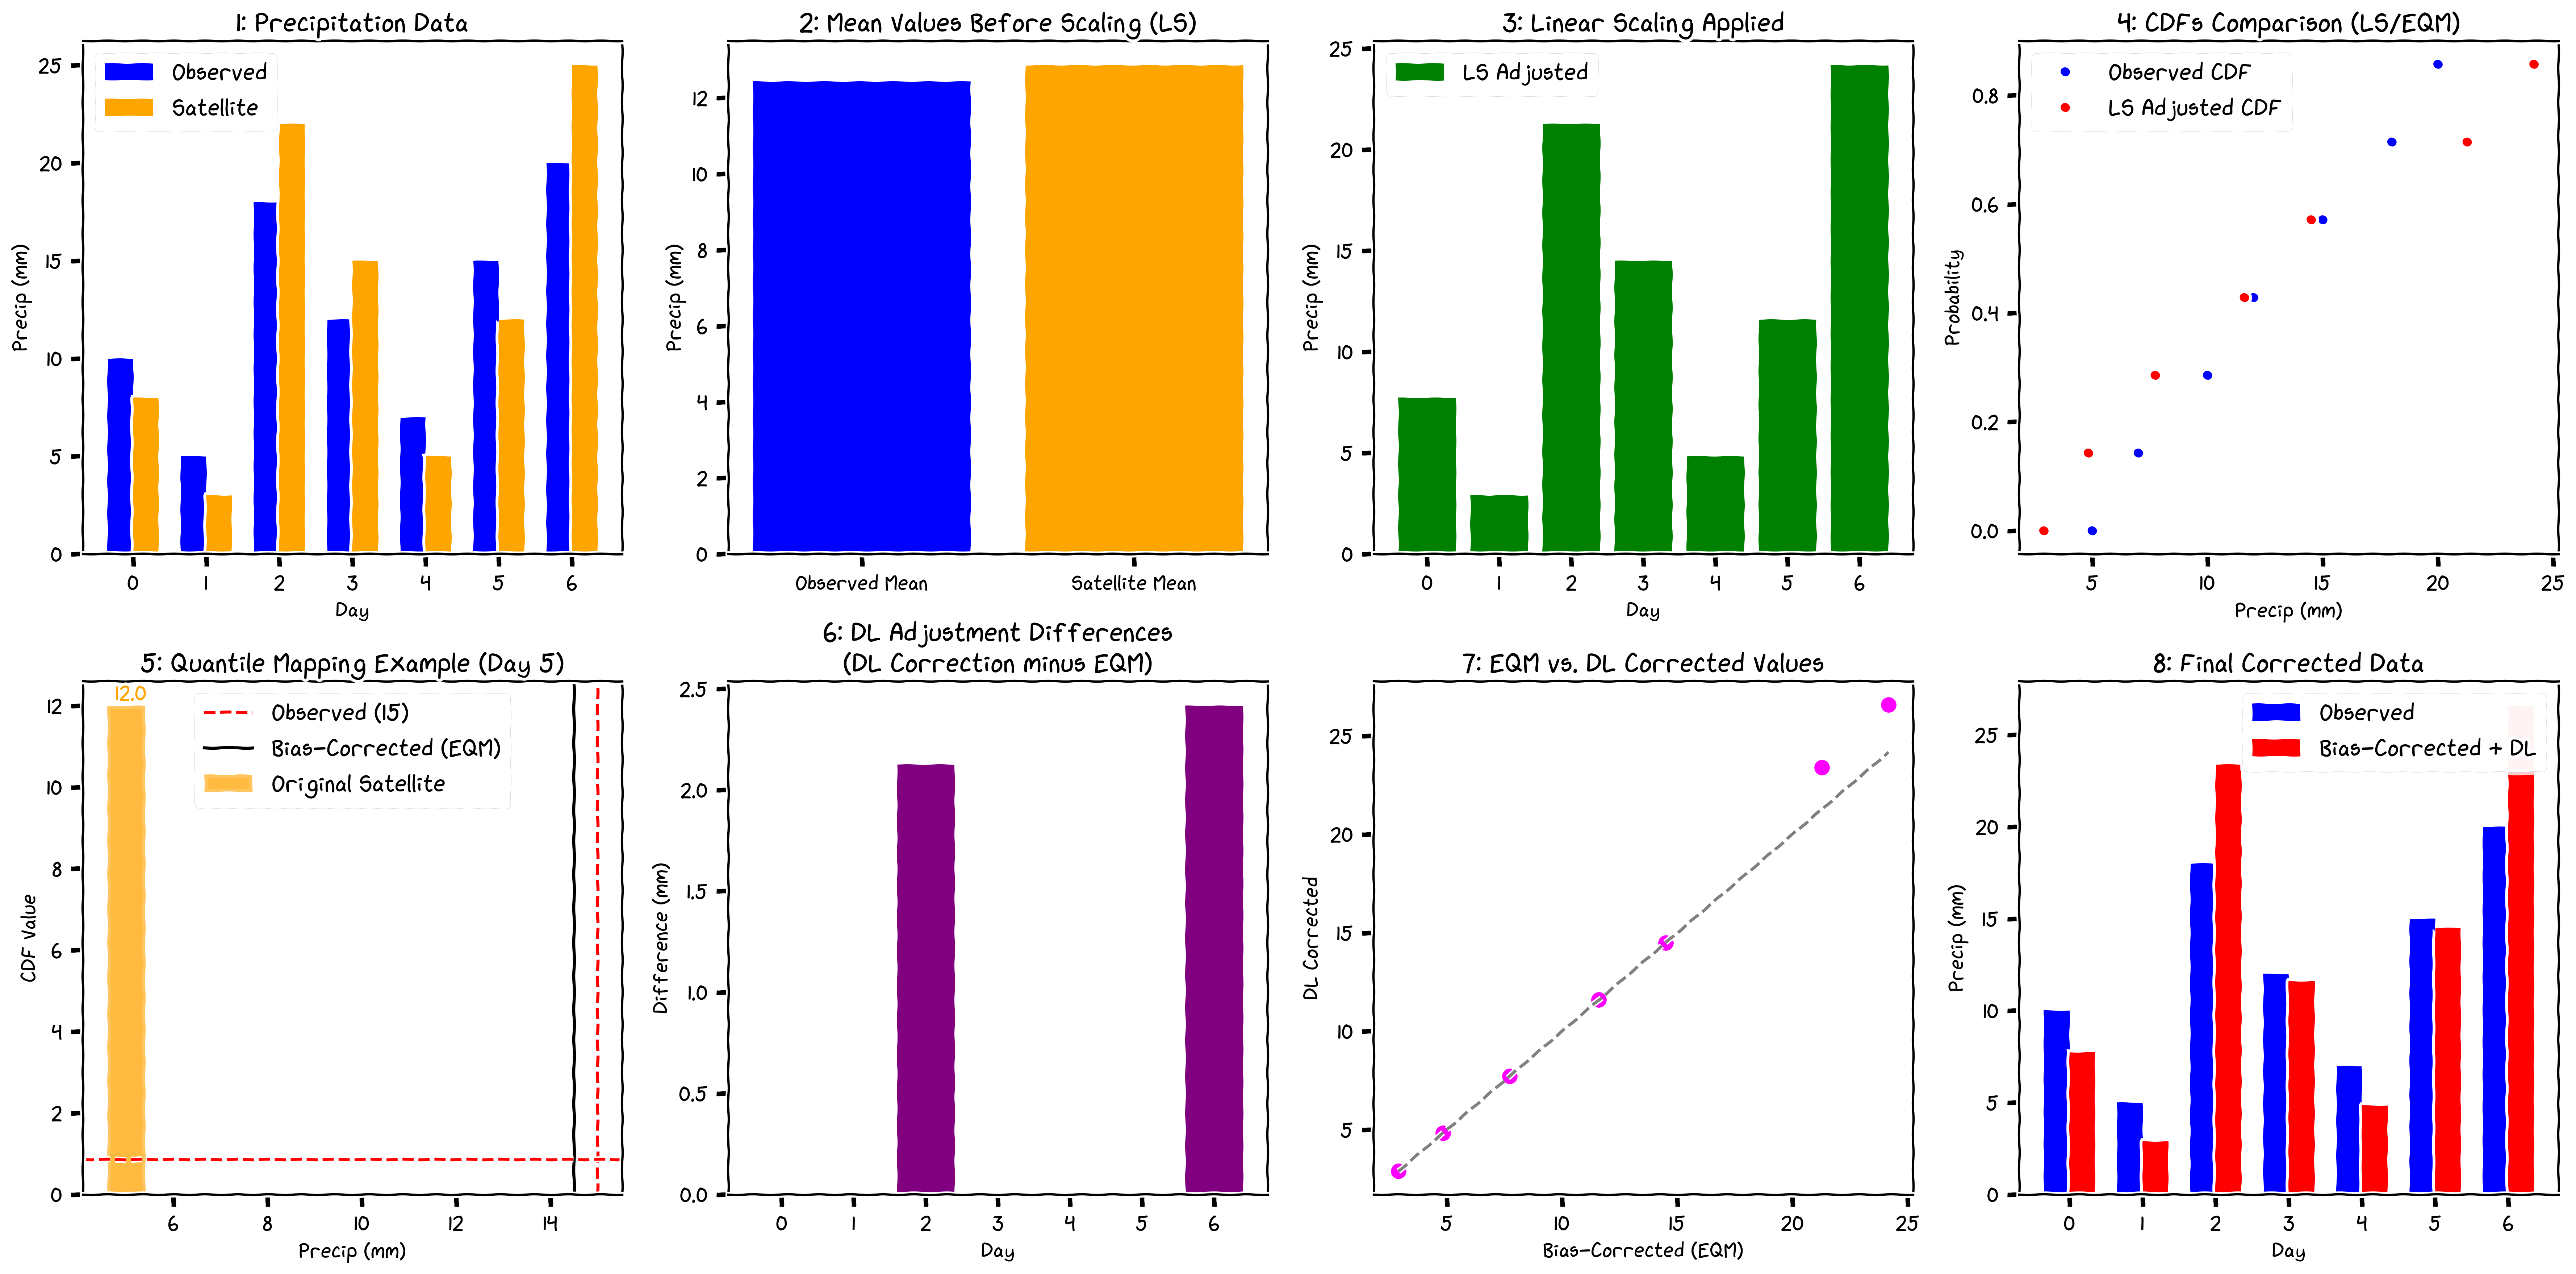
\includegraphics[width=\textwidth]{images/fig01_framework.png}
\caption{Conceptual workflow of the LSEQM+DL hybrid bias correction framework.\label{fig1}}
\end{figure}

\subsection{Study Region}\label{study-region}

Indonesia (95--141\textdegree E, 11\textdegree S--6\textdegree N), the world's largest archipelagic country, presents a complex
and challenging environment for precipitation estimation. Located
between the Indian and Pacific Oceans and straddling the equator,
Indonesia experiences a tropical climate characterized by high spatial
and temporal variability in rainfall \cite{ref19,ref20}. Topographical
diversity, ranging from lowland plains to mountainous regions exceeding
4,000 meters in elevation, further complicates precipitation patterns.
The country is highly vulnerable to extreme rainfall events that
frequently trigger flooding, landslides, and other hydrometeorological
disasters.

This study adopts Indonesia as the area of interest (AOI) due to its
critical need for improved precipitation monitoring and its
representative challenges for satellite-based hydrometeorological
applications. While the Indonesia's Meteorological, Climatological, and
Geophysical Agency (BMKG) station data used for validation are specific
to Indonesia, the primary datasets utilized for bias correction, IMERG
and CPC-UNI, are globally available. Moreover, the methodology does
not embed Indonesia-specific structural assumptions; the GPD threshold,
blending weight, and saturation count would require regional
recalibration, but the cascade itself is portable. Within Indonesia,
the gauge-density gradient between Java and the eastern provinces
provides a within-domain test of how the framework behaves at both
ends of the data-availability spectrum.

\subsection{Data and Preprocessing}\label{data-and-preprocessing}

Three precipitation datasets are used in this study \cite{ref22}. The IMERG Late Run (IMERG-L; 0.1\textdegree, \textasciitilde14-hour latency) \cite{ref2,ref21} serves as the satellite product to be corrected; because IMERG-L relies purely on satellite observations without gauge assimilation, it provides an uncontaminated baseline for evaluating bias correction. The IMERG Final Run (IMERG-F; 0.1\textdegree) \cite{ref2}, which incorporates gauge data during post-processing, is included as an independent evaluation benchmark but is not used in the correction procedure. The CPC Unified Gauge-Based Analysis of Global Daily Precipitation (CPC-UNI; 0.5\textdegree) \cite{ref13,ref18} serves as the reference for bias correction. CPC-UNI is the highest-resolution global daily gauge-analysis product, though its interpolated values may not capture local extremes in regions with sparse station networks. All satellite data were obtained from the NASA GES DISC; CPC-UNI from the NOAA Physical Sciences Laboratory.

Independent validation uses daily observations from 171 stations operated by Indonesia's Meteorological, Climatological, and Geophysical Agency (BMKG). These station observations are not used in the distributional fitting (LS, EQM, GPD) or in CNN training, and the validation is therefore independent of the value-based correction stages. Station locations from the BMKG network also inform the construction of the station density confidence mask (Section~\ref{stage-4-dl}); the validation thus uses observation values that did not enter the correction pipeline, while location information overlapping with the validation set contributes to the mask design. Strict location-disjoint validation is left to future work.

Prior to correction, datasets were harmonized through spatial regridding (CPC-UNI to the IMERG grid via nearest-neighbor interpolation), temporal alignment, land-sea masking, and latitude reindexing. Following the Bias Correction Spatial Disaggregation (BCSD) principle \cite{ref23}, statistical fields are estimated at the native 0.5\textdegree{} CPC-UNI resolution and bilinearly interpolated to 0.1\textdegree{} before being applied: the LS scaling factor uses dekadal mean precipitation, EQM uses fitted gamma parameters \((k, \theta)\), and GPD uses fitted shape, scale, and threshold parameters \((\xi, \sigma, u)\). A wet-day threshold of 1.0 mm/day is applied throughout, consistent with WMO recommendations for tropical regions \cite{ref24}. Full preprocessing details are provided in Supplementary S1.

\subsection{Hybrid Bias Correction
Methodology}\label{hybrid-bias-correction-methodology}

The operational implementation follows a sequential four-stage structure.
Each processing stage targets a specific source of bias in
satellite-derived daily precipitation estimates. All bias correction
steps are performed separately for each dekadal period (three
subdivisions per month: days 1--10, 11--20, and 21 to end of month).
Within each dekad, daily precipitation values are pooled across all
available years (2001--2025), yielding approximately 230 samples per
dekad. This multi-year pooling strategy enhances the statistical
robustness of distribution fitting and extreme value estimation, while
preserving the seasonal characteristics of each dekadal window.

The overall hybrid bias correction workflow is illustrated in \hyperref[fig2]{Figure~2}.

\begin{figure}[H]
\centering
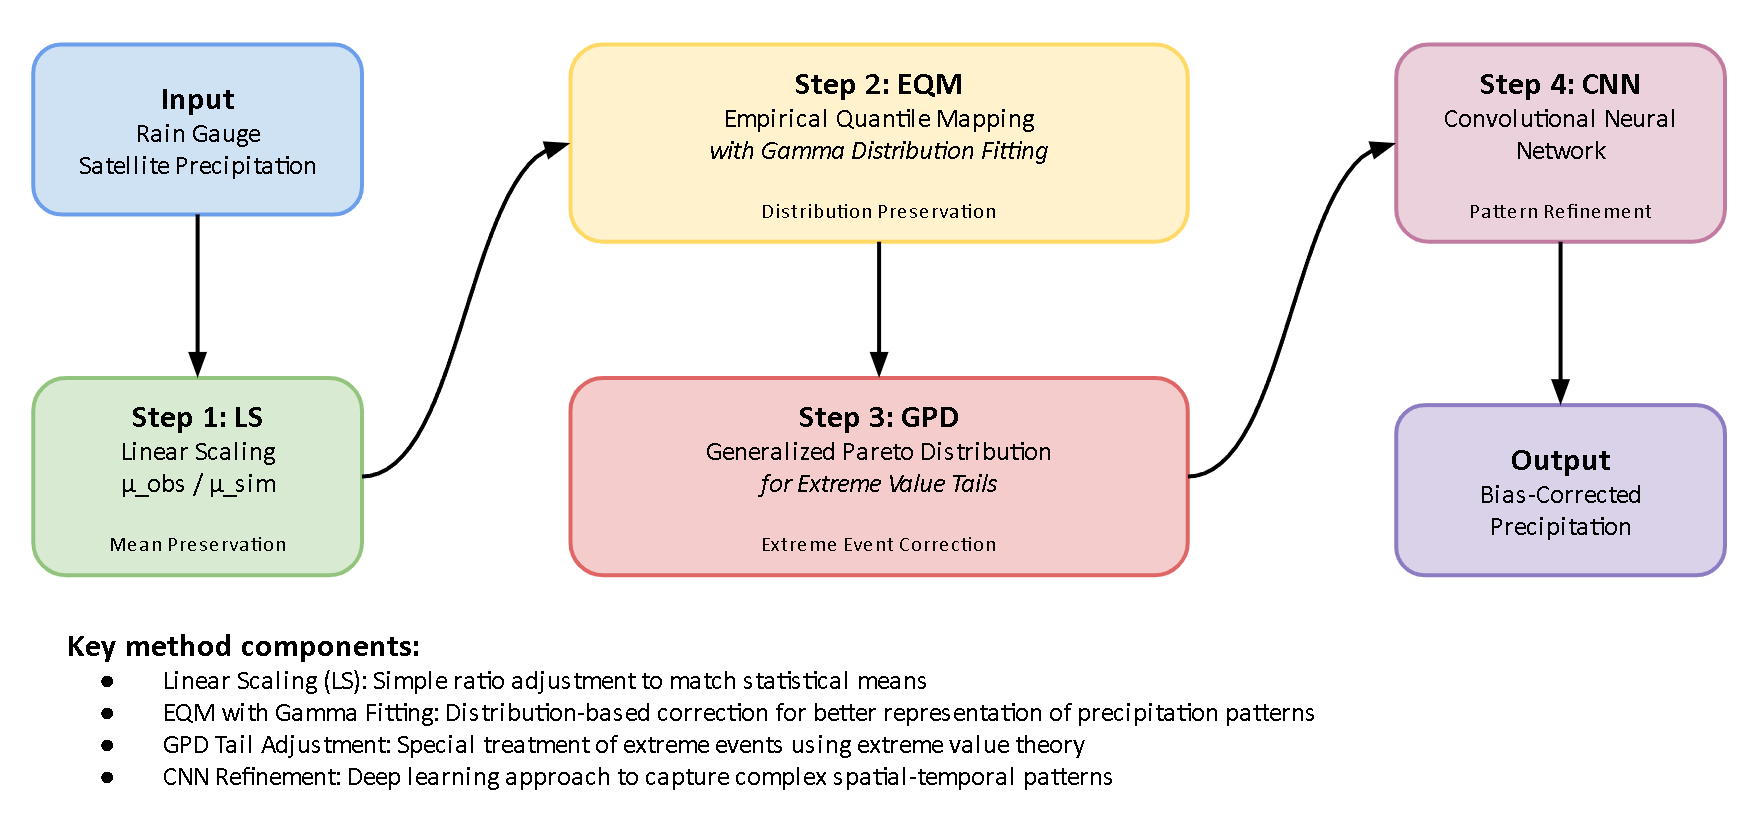
\includegraphics[width=\textwidth]{images/fig02_workflow.png}
\caption{Overview of the hybrid bias correction workflow integrating Linear Scaling (LS), Empirical Quantile Mapping (EQM) with Gamma fitting, Generalized Pareto Distribution (GPD) tail adjustment, and Convolutional Neural Network (CNN) refinement.\label{fig2}}
\end{figure}

\subsubsection{Stage 1: Linear Scaling}\label{stage-1-linear-scaling}

Linear Scaling corrects the systematic mean bias by applying a
multiplicative factor derived from the ratio of reference to satellite
mean precipitation. For each dekad, the scaling factor \(C_{LS}\) is
computed as:

\begin{equation}C_{LS} = \frac{\bar{P}_{ref}}{\bar{P}_{sat}}\end{equation}

where \(\bar{P}_{ref}\) and \(\bar{P}_{sat}\) are the mean daily
precipitation of the CPC-UNI reference and IMERG-L satellite datasets,
respectively, pooled over the same dekadal period across all years. The
corrected precipitation is:

\begin{equation}P_{LS} = P_{sat} \cdot C_{LS}\end{equation}

Grid cells where the satellite mean is zero are left unchanged. Following the BCSD strategy (\hyperref[data-and-preprocessing]{Section~2.2}), \(\bar{P}_{ref}\) is computed at the native \(0.5^{\circ}\) CPC-UNI grid and bilinearly interpolated to \(0.1^{\circ}\), producing a spatially smooth scaling field.

\subsubsection{Stage 2: Empirical Quantile Mapping with Gamma Distribution Fitting (EQM)}\label{stage-2-eqm}

Empirical Quantile Mapping aligns the full cumulative distribution
function (CDF) of the LS-corrected satellite precipitation to that of
the reference observations. To improve the stability and smoothness of
the CDFs, particularly in regions with limited sample sizes, gamma
distributions are fitted to the precipitation data prior to mapping.
Gamma parameters (shape \(k\) and scale \(\theta\)) are estimated using
maximum likelihood estimation (MLE) with the location parameter fixed at
zero to ensure physical validity of non-negative precipitation values
\cite{ref15}. The quantile correction for each satellite precipitation value
\(P_{LS}\) is performed by:

\begin{equation}P_{EQM} = F_{ref}^{-1}\left( F_{sat}\left( P_{LS} \right) \right)\end{equation}

where \(F_{sat}\) and \(F_{ref}\) denote the fitted gamma CDFs of the
satellite and reference datasets, respectively, and \(F_{ref}^{-1}\) is
the inverse CDF (quantile function) of the reference distribution.

The satellite-side gamma CDF is fitted independently at each \(0.1^{\circ}\) pixel, while the reference gamma CDF is fitted at the native \(0.5^{\circ}\) CPC-UNI resolution and the parameters bilinearly interpolated to \(0.1^{\circ}\), consistent with the BCSD strategy \cite{ref23}.

\paragraph{Dry-day handling} Because daily tropical precipitation is a
mixed discrete-continuous variable with a large atom at zero, the gamma
distribution is fitted only on wet days (\(P \geq 1\) mm/day) rather
than on the full sample. Fitting a gamma to the mixed sample would bias
the shape parameter toward zero and distort the mapped quantiles. The
dry-day fraction is handled explicitly at the mapping stage following
the unconditional-CDF construction of Cannon et al.~\cite{ref11}. Let
\(p_{dry}^{sat}\) and \(p_{dry}^{ref}\) denote the satellite and
reference dry-day probabilities estimated at each pixel from the
empirical sample. For a satellite wet-day value \(P_{LS} \geq 1\)
mm/day, the unconditional quantile position is
\begin{equation}y = p_{dry}^{sat} + (1 - p_{dry}^{sat}) \cdot F_{sat}^{wet}(P_{LS}),\end{equation}
where \(F_{sat}^{wet}\) is the gamma CDF fitted on wet values only. The
reference quantile is then obtained from the analogous reference
unconditional CDF, with values falling below \(p_{dry}^{ref}\) mapped to
zero. This construction preserves the reference dry-day frequency by
design and prevents satellite drizzle from being mapped to spurious
low-intensity wet-day values.

\subsubsection{Stage 3: Generalized Pareto Distribution (GPD) Tail Adjustment}\label{stage-3-gpd}

Extreme precipitation values are modeled separately to preserve the
frequency and magnitude of high-impact events that gamma-based EQM may
underrepresent. Precipitation exceedances above the 80th percentile of
the wet-day sample are fitted using the Generalized Pareto Distribution,
with separate thresholds \(u_{sat}\) and \(u_{ref}\) estimated from the
satellite and reference wet-value distributions, respectively. The 80th
percentile threshold was selected to balance two competing requirements:
a sufficiently large number of exceedances for stable GPD parameter
estimation, and a threshold high enough to isolate genuinely extreme
behavior from the bulk distribution \cite{ref7}. This threshold is
consistent with recommendations for tropical regions with frequent heavy
rainfall, where lower thresholds risk contaminating GPD fits with
moderate rainfall, while higher thresholds yield too few exceedances for
reliable estimation \cite{ref25}.

For precipitation values exceeding threshold \(u\), the exceedances
\(y = P - u\) are modeled using the GPD probability density function:

\begin{equation}f(y) = \frac{1}{\sigma} \left( 1 + \xi \frac{y}{\sigma} \right)^{-(1 + 1/\xi)}, \qquad y \geq 0,\; 1 + \xi y/\sigma > 0\end{equation}

with the limiting case \(\xi = 0\) corresponding to the exponential distribution \(f(y) = (1/\sigma) \exp(-y/\sigma)\).

where \(\xi\) is the shape parameter and \(\sigma\) is the scale
parameter. The location parameter is fixed at zero because exceedances
are non-negative by construction; leaving the location free would bias
the fitted tail \cite{ref7}. To improve robustness against data sparsity,
GPD parameters are estimated using \(K\)-fold cross-validation
(\(K = 5\)) with shuffled folds, and the final parameters are averaged
across all folds to reduce sensitivity to individual outliers \cite{ref25}.
Conditional probability mapping is then applied to correct extreme
quantiles. For an LS-corrected value \(P_{LS} > u_{sat}\), the conditional
exceedance probability is computed on the satellite side using its own
threshold,

\begin{equation}p_c = \frac{F_{sat}(P_{LS}) - F_{sat}(u_{sat})}{1 - F_{sat}(u_{sat})},\end{equation}

and the GPD-corrected value is obtained from the reference GPD as

\begin{equation}P_{LSEQM} = u_{ref} + G_{ref}^{-1}(p_c),\end{equation}

where \(G_{ref}^{-1}\) is the inverse GPD fitted to the reference
exceedances and \(u_{ref}\) is the reference wet-value 80th percentile.
Computing \(p_c\) on the satellite side keeps the
tail-substitution probability chain is internally consistent with the
unconditional gamma CDF used in the body of the distribution, and
maintains continuity at the gamma-GPD boundary.

As with the gamma parameters, GPD parameters are fitted at the native \(0.5^{\circ}\) resolution and interpolated to \(0.1^{\circ}\). Corrected values are capped at the interpolated 99.9th percentile of the reference distribution to prevent physically unrealistic extremes from GPD extrapolation.

\subsubsection{Stage 4: Deep Learning Refinement (CNN)}\label{stage-4-dl}

Although the preceding statistical corrections substantially reduce
biases in mean, distribution, and extremes, residual errors in extreme
precipitation pixels often persist due to complex local topographic and
atmospheric processes. To address these remaining biases, a
Convolutional Neural Network (CNN) is employed to refine the corrected
precipitation fields, with its corrections selectively applied to
extreme pixels through alpha-blending.

The CNN is trained separately for each dekadal period, using the
LSEQM-corrected fields as input and CPC-UNI observations as the training
target. This two-stage design means the CNN receives input from the same
statistical domain at both training and inference time, avoiding the
domain shift problem that arises when training directly on raw satellite
data \cite{ref9}.

Each daily precipitation field is independently normalized to \([0, 1]\) by dividing by its spatial maximum. The CNN comprises two convolutional blocks (\(3 \times 3\) filters, 32/64 channels) with max pooling and dropout, followed by a Flatten-Dense bottleneck (128 units) and a linear output layer (\hyperref[fig3]{Figure~3}). The model is trained by minimizing mean squared error using the Adam optimizer \cite{ref26} with early stopping (patience = 5 epochs) and an 80/20 training-validation split. For the Indonesia domain (170 latitude \(\times\) 460 longitude pixels at \(0.1^{\circ}\)), this architecture comprises tens of millions of trainable parameters, dominated by the Dense reconstruction layer. The parameter-to-sample ratio relative to the daily fields available per dekad motivates the conservative blending cap (\(\alpha = 0.70\)) and the extreme-pixel-only application of CNN outputs (Section below) as overfitting safeguards beyond the dropout regularization.

\begin{figure}[H]
\centering
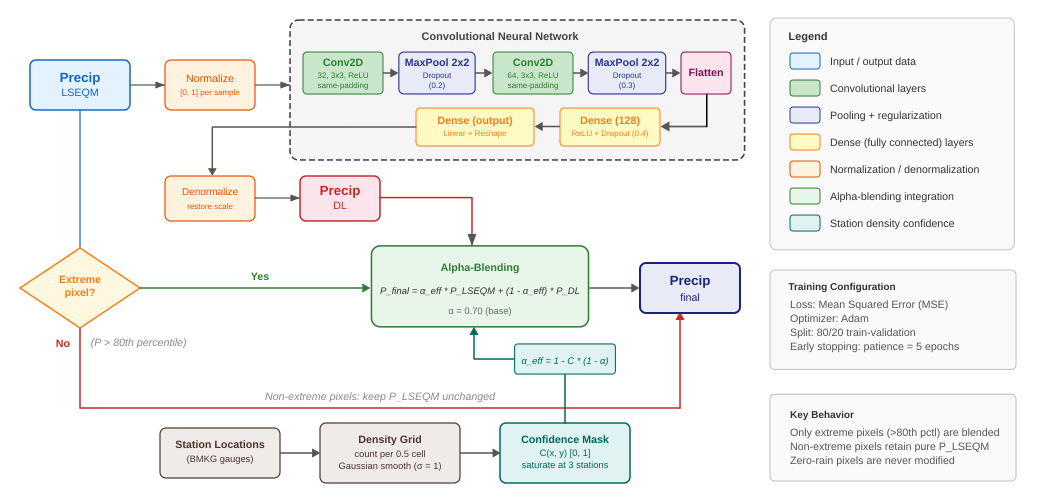
\includegraphics[width=\textwidth]{images/fig03_cnn_pipeline.png}
\caption{CNN refinement pipeline: LSEQM-corrected daily fields are normalized, passed through two convolutional blocks and a Flatten-Dense bottleneck, and reconstructed as a refined field. The refined field is then combined with the LSEQM field through the station-density-modulated alpha-blending step applied only to pixels exceeding the 80th percentile.\label{fig3}}
\end{figure}

\paragraph{Alpha-Blending Integration}

The CNN predictions are not applied uniformly across all grid cells.
Instead, an alpha-blending strategy selectively integrates the DL
refinement with the statistical corrections. For each grid cell and time
step, the final corrected precipitation is:

\begin{equation}P_{final} = \alpha_{eff} \cdot P_{LSEQM} + (1 - \alpha_{eff}) \cdot P_{DL}\end{equation}

where \(\alpha_{eff}\) is the effective blending weight. This blending
is applied only to pixels identified as extreme, defined as those where
\(P_{LSEQM}\) exceeds the 80th percentile of the pixel's dekadal
distribution.

Non-extreme pixels retain their LSEQM values without modification, and
pixels with zero precipitation are preserved as zero. The base blending
weight \(\alpha = 0.70\) assigns 70\% weight to the physical-statistical
correction and 30\% to the DL refinement.

\paragraph{Station Density Confidence Weighting}

The reliability of the CPC-UNI reference varies spatially depending on
the density of contributing gauge stations. To account for this
heterogeneity, a station density confidence mask modulates the blending
parameter. Gauge station counts per CPC-UNI native grid cell
(\(0.5^{\circ}\)) are computed from the BMKG station network,
Gaussian-smoothed (\(\sigma = 1.0\) grid cells) to prevent sharp
boundaries, then normalized to \([0, 1]\) by dividing by a saturation
count of 2 stations per cell. The confidence mask \(C(x, y)\) modulates
the blending parameter as:

\begin{equation}\alpha_{eff}(x, y) = 1.0 - C(x, y) \cdot (1.0 - \alpha)\end{equation}

This formulation provides a smooth spatial transition: station-dense
areas receive the full DL contribution (\(\alpha_{eff} = 0.70\)), while
station-sparse areas revert toward pure LSEQM
(\(\alpha_{eff} \rightarrow 1.0\)). This approach reduces the risk of
the DL model introducing artifacts in regions where the training target
itself is uncertain \cite{ref27}.

\subsection{Model Evaluation and Quality
Assessment}\label{model-evaluation-and-quality-assessment}

Evaluating bias correction of daily precipitation requires a
multi-metric framework that captures statistical accuracy,
distributional consistency, temporal pattern preservation, and the
representation of extreme events. Daily precipitation exhibits high
temporal variability, frequent dry periods, and intermittent extreme
events, making it more difficult to evaluate than monthly-aggregated
precipitation. A single performance metric cannot capture correction
quality across all relevant dimensions (event timing, intensity
distribution, dry spell behavior, and extremes), and this study
therefore employs a structured suite of statistical, categorical,
temporal, and distributional metrics combined with integrated quality
indices, consistent with recommended practice for satellite
precipitation verification \cite{ref14,ref15}.

\subsubsection{Nine-Combination Evaluation Design}\label{nine-combination-evaluation-design}

The evaluation follows a systematic 3 x 3 factorial design (\hyperref[tab:1]{Table~1}).
Three reference datasets are used: (1) CPC-UNI, the gauge-based product
used as the training reference for bias correction; (2) IMERG-L, the
uncorrected satellite product; and (3) IMERG-F, the gauge-adjusted IMERG
Final Run product, which serves as an independent benchmark. Each
reference is compared against three correction stages: LS (mean
correction only), LSEQM (mean + distributional correction), and LSEQM+DL
(full hybrid correction). This yields nine reference-test combinations,
enabling three complementary perspectives:

\begin{itemize}
\tightlist
\item
  \textbf{CPC-UNI vs.~corrected products:} Measures absolute correction
  quality against the training reference, assessing how well each stage
  reproduces the gauge-based observations.
\item
  \textbf{IMERG-L vs.~corrected products:} Quantifies improvement
  relative to the uncorrected satellite baseline, isolating the added
  value of bias correction.
\item
  \textbf{IMERG-F vs.~corrected products:} Evaluates performance against
  an independent, gauge-adjusted satellite product that was not used in
  the correction procedure, providing a less circular validation.
\end{itemize}

\phantomsection\label{tab:1}
\textbf{Table 1.} Evaluation matrix: nine reference-test combinations.

\begingroup\small
\begin{longtable}[]{@{}llll@{}}
\toprule
& \textbf{LS} & \textbf{LSEQM} & \textbf{LSEQM+DL} \\
\midrule
\endhead
\bottomrule
\endlastfoot
\textbf{CPC-UNI} & CPC-UNI vs LS & CPC-UNI vs LSEQM & CPC-UNI vs
LSEQM+DL \\
\textbf{IMERG-L} & IMERG-L vs LS & IMERG-L vs LSEQM & IMERG-L vs
LSEQM+DL \\
\textbf{IMERG-F} & IMERG-F vs LS & IMERG-F vs LSEQM & IMERG-F vs
LSEQM+DL \\
\end{longtable}
\endgroup

\subsubsection{Evaluation Metrics}\label{evaluation-metrics}

Correction performance is evaluated using 31 verification metrics organized into four categories (\hyperref[tab:2]{Table~2}): continuous statistical measures (Relative Bias, Pearson Correlation, RMSE, MAE, NSE, Standard Deviation Ratio, KS test), categorical event detection (POD, FAR, CSI, ETS), temporal pattern fidelity (Frequency of Precipitation Days, Mean Wet-Day Precipitation, Maximum Dry Spell Length), and distributional consistency (six percentiles from \(Q_{25}\) to \(Q_{99}\)). All metrics are computed at the pixel level for each dekadal period, following established definitions \cite{ref14,ref15,ref28,ref29}. Mathematical formulas for all metrics are provided in Supplementary S2.

\phantomsection\label{tab:2}
\textbf{Table 2.} Summary of verification metrics.

\begingroup\small
\begin{longtable}[]{@{}llccc@{}}
\toprule
Category & Metric & Abbreviation & Unit & Perfect Score \\
\midrule
\endhead
\bottomrule
\endlastfoot
Continuous & Relative Bias & RB & ratio & 0 \\
& Pearson Correlation & CORR & -- & 1 \\
& Root Mean Square Error & RMSE & mm/day & 0 \\
& Mean Absolute Error & MAE & mm/day & 0 \\
& Nash-Sutcliffe Efficiency & NSE & -- & 1 \\
& Standard Deviation (ref, test) & STDEV & mm/day & equal \\
& Standard Deviation Ratio & SDR & ratio & 1 \\
& KS Test Statistic / \(p\)-value & KS & -- & 0 / 1 \\
Categorical & Probability of Detection & POD & -- & 1 \\
& False Alarm Ratio & FAR & -- & 0 \\
& Critical Success Index & CSI & -- & 1 \\
& Equitable Threat Score & ETS & -- & 1 \\
Temporal & Frequency of Precipitation Days & FPD & \% & equal \\
& Mean Wet-Day Precipitation & MDWP & mm/day & equal \\
& Maximum Dry Spell Length & DSL & days & equal \\
Distributional & Percentiles (\(Q_{25}\) -- \(Q_{99}\)) & \(Q_{xx}\) &
mm/day & equal \\
\end{longtable}
\endgroup

\subsubsection{Composite Quality Assessment Framework}\label{composite-quality-assessment-framework}

To evaluate overall correction quality across multiple dimensions simultaneously, the Continuous Quality Index (CQI) aggregates individual metrics into three principal component scores \cite{ref30}:

\begin{equation}\text{BSQS} = 0.30 \cdot S_{RB} + 0.30 \cdot S_{RMSE} + 0.40 \cdot S_{NSE}\end{equation}

\begin{equation}\text{DQS} = 0.45 \cdot S_{extreme} + 0.25 \cdot S_{general} + 0.15 \cdot S_{var} + 0.15 \cdot S_{KS}\end{equation}

\begin{equation}\text{TQS} = 0.40 \cdot S_{CSI} + 0.30 \cdot S_{event} + 0.30 \cdot S_{spell}\end{equation}

where BSQS captures basic statistical accuracy (bias, error magnitude, prediction efficiency), DQS evaluates distributional preservation with emphasis on extreme percentiles (weight 0.45), and TQS assesses temporal pattern fidelity including event detection and dry spell persistence. The overall CQI synthesizes these components:

\begin{equation}\text{CQI} = 0.35 \cdot \text{BSQS} + 0.35 \cdot \text{DQS} + 0.30 \cdot \text{TQS}\end{equation}

CQI values are classified as Excellent (\(\geq 0.8\)), Good (\(0.6\text{--}0.8\)), Fair (\(0.4\text{--}0.6\)), or Poor (\(< 0.4\)). Because the majority of pixels fall within the Fair range, \hyperref[fig7]{Figure~7b} employs a finer six-tier subdivision to reveal spatial structure. Sub-score formulas and the full classification table are provided in Supplementary S2.

A pixel-level confidence score, based on metric consistency and distributional agreement, flags regions where the evaluation may be less reliable due to data limitations. The confidence formulation is detailed in Supplementary S3.

\section{Results and Discussion}\label{results-and-discussion}

Before examining correction performance, it is important to characterize
the starting conditions. The uncorrected IMERG Late Run over Indonesia
exhibits a systematic wet bias against the CPC-UNI reference, with
domain-median relative bias of approximately +15.5\% during the wet season
(October--March). This bias has a conditional structure: IMERG
overestimates precipitation on days that CPC-UNI classifies as light
rain while simultaneously underestimating moderate-to-heavy events
(\hyperref[progressive-improvement]{Section~3.1}), a pattern consistent with published IMERG-L evaluations
over the Maritime Continent \cite{ref31,ref32,ref33}. The CPC-UNI reference itself
carries important limitations: at \(0.5^{\circ}\) resolution with 180
contributing stations across Indonesia, gauge density is heavily
concentrated in Java and southern Sumatra (\hyperref[role-station-density]{Section~3.6}, Figure 10a),
leaving eastern Indonesia (Papua, Maluku, Nusa Tenggara) dependent on
interpolation that may not capture local extremes. The independent BMKG
station network used for validation (171 stations with \(\geq\) 30 valid
days) shares a similar spatial distribution, with station density
highest in Java. This geographic concentration means that domain-median
validation statistics are more representative of conditions in
station-dense western Indonesia than in the data-sparse east, a
caveat that should be borne in mind when interpreting the results below.

\subsection{Progressive Improvement Across Correction
Stages}\label{progressive-improvement}

The hybrid framework targets three complementary aspects of satellite
precipitation bias: adjusting values (mean and magnitude), aligning
distributions (statistical shape), and preserving extremes (tail
accuracy). To evaluate whether each correction stage delivers on its
intended objective, domain-wide verification metrics were computed for
the uncorrected IMERG Late Run and the three correction products (LS,
LSEQM, and LSEQM+DL) against the CPC-UNI gauge-based reference. \hyperref[tab:3]{Table~3}
organizes the evaluation around these three design objectives,
supplemented by categorical event detection metrics. All values
represent the spatial median across Indonesian land pixels, averaged
over 36 dekadal periods (12 months \(\times\) 3 dekads per month). Ratio
metrics express the corrected product relative to the reference (target
= 1.0).

\begin{landscape}
\phantomsection\label{tab:3}
\textbf{Table 3.} Domain-wide evaluation by correction stage against
CPC-UNI, organized by the three design objectives of the hybrid
framework. Values represent the spatial median across all land pixels,
averaged over all 36 dekadal periods. Ratio metrics express
test/reference. Bold indicates the value closest to the target.

\begingroup\small
\begin{longtable}[]{@{}llllll@{}}
\toprule
Evaluation Objective & Metric & LS & LSEQM & LSEQM+DL & Target \\
\midrule
\endhead
\bottomrule
\endlastfoot
\textbf{Value Adjustment} & Relative Bias & 0.0000 & 0.0697 & 0.0652 &
0 \\
& Std. Dev. Ratio & 0.9707 & 1.1587 & 1.1475 & 1.0 \\
\textbf{Distribution Alignment} & KS \(p\)-value (\%) & 6.56 & 0.00 &
0.00 & 100 \\
& Wet-Day Freq. Ratio & 1.0397 & 0.9466 & 0.9462 & 1.0 \\
& Mean Wet-Day Precip Ratio & 0.9611 & 1.1569 & 1.1519 & 1.0 \\
\textbf{Extreme Preservation} & \(Q_{95}\) Ratio & 0.9459 & 1.1711 &
1.1626 & 1.0 \\
& \(Q_{99}\) Ratio & 0.9669 & 1.2117 & 1.1964 & 1.0 \\
\textbf{Event Detection} & POD & 0.7669 & 0.7069 & 0.7069 & 1.0 \\
& CSI & 0.5890 & 0.5723 & 0.5724 & 1.0 \\
& FAR & 0.2705 & 0.2476 & 0.2475 & 0 \\
\textbf{Temporal Skill} (acknowledged limitation) & Pearson Corr &
0.3430 & 0.3451 & 0.3476 & 1.0 \\
& RMSE (mm/day) & 13.1051 & 14.1797 & 14.0717 & 0 \\
& NSE & $-$0.2728 & $-$0.5479 & $-$0.5241 & 1.0 \\
\end{longtable}
\endgroup
\end{landscape}

The results reveal a pattern consistent with the design intent of each
correction stage. Linear Scaling drives the domain-wide relative bias
against CPC-UNI to zero by construction, since \(C_{LS}\) is defined
exactly as the ratio of reference to satellite dekadal means; the
standard deviation ratio of \(\approx 0.97\) indicates that a uniform
multiplicative rescaling leaves the distributional shape essentially
unchanged. The addition of EQM with GPD tail adjustment (LSEQM) then
modifies the shape of the distribution: the wet-day-mean ratio moves
from 0.96 (LS) to 1.16 and the \(Q_{95}\)/\(Q_{99}\) ratios move from
below unity to above unity (\hyperref[tab:3]{Table~3}). These shifts are intentional
rather than deficient: LS by construction under-represents wet-day
intensity because it also rescales drizzle days upward, and EQM with a
wet-day-only gamma fit plus explicit dry-day handling (\hyperref[hybrid-bias-correction-methodology]{Section~2.3})
lifts the conditional wet-day distribution back toward the reference.
The apparent ``overshoot'' at the upper percentiles against CPC-UNI is
analyzed further in \hyperref[station-level-ground-truth-validation]{Section~3.5} and \hyperref[discussion]{Section~3.8}, where independent BMKG
station validation shows that the LSEQM+DL \(Q_{99}\) ratio lands at
1.01 against gauge observations, compared with 0.71 for LS, the
opposite direction from the CPC-UNI-based assessment.

The CNN refinement (LSEQM+DL) provides targeted adjustment at the
extreme end: the standard deviation ratio moves slightly closer to unity
and \(Q_{95}\)/\(Q_{99}\) move modestly toward the reference. The CNN
effect is intentionally small, reflecting the conservative
alpha-blending design (\(\alpha = 0.70\) applied only to extreme
pixels), which limits the DL contribution to at most 30\% of the
correction signal and only where the station density confidence mask
permits.

Event detection shows a trade-off inherent to distributional correction:
POD and CSI shift marginally across correction stages (\hyperref[tab:3]{Table~3}),
reflecting the fact that quantile mapping adjusts wet-day precipitation
magnitudes and can move marginal events above or below the 1 mm/day
detection threshold. FAR remains essentially unchanged, indicating that
the redistribution of values does not systematically inflate false
alarms.

An important characteristic of distributional bias correction methods is
that they adjust marginal distributions without modifying the temporal
sequencing of satellite estimates \cite{ref34,ref11}. Accordingly, pixel-level
temporal accuracy metrics show limited change across correction stages:
Pearson correlation remains at approximately 0.35, RMSE at approximately
13 mm/day, and NSE remains negative (approximately \(-0.3\)) for all
methods. These values reflect the inherent difficulty of reproducing
gauge-interpolated daily precipitation fields at 0.1\(^{\circ}\)
resolution rather than a deficiency of the correction framework. The
method is designed to produce climatologically unbiased rainfall fields
with correct distributional properties (adjusting values, aligning
distributions, and preserving extremes) rather than to improve
day-to-day prediction skill at the pixel level.

To provide a compact visual summary of these multi-dimensional
performance characteristics, \hyperref[fig4]{Figure~4} presents Taylor diagrams \cite{ref35}
comparing all evaluated products against independent BMKG station
observations, stratified by monsoon regime. The diagram simultaneously
displays three complementary statistics: Pearson correlation (angular
position), normalized standard deviation (radial distance), and centered
RMSE (gray dashed contours). A product that perfectly reproduces the
observed variability would coincide with the reference point at
correlation = 1.0 and normalized standard deviation = 1.0.

The seasonal stratification reveals that the method ordering is stable
across both monsoon regimes. In both wet (October--March) and dry
(April--September) seasons, LS underestimates the observed variability
(median standard deviation ratio of 0.71 and 0.74, respectively), while
LSEQM and LSEQM+DL bring the ratio toward unity (1.03/1.00 in the wet
season, 1.04/1.02 in the dry season). Correlation remains largely
unchanged across correction stages (\(\approx\) 0.22--0.25), confirming
that distributional correction does not modify temporal prediction skill,
consistent with the theoretical expectation discussed in \hyperref[discussion]{Section~3.8}. CPC-UNI, despite serving as the correction target, does not
coincide with the station reference point (standard deviation ratio
\(\approx\) 0.85), reflecting the interpolation uncertainty inherent to
the gauge analysis at \(0.5^{\circ}\) resolution, a characteristic
that motivates the independent station validation. IMERG-F, included as
an independent benchmark, sits between the uncorrected IMERG-L and the
CPC-UNI reference, consistent with its gauge-adjusted nature.

\begin{figure}[H]
\centering
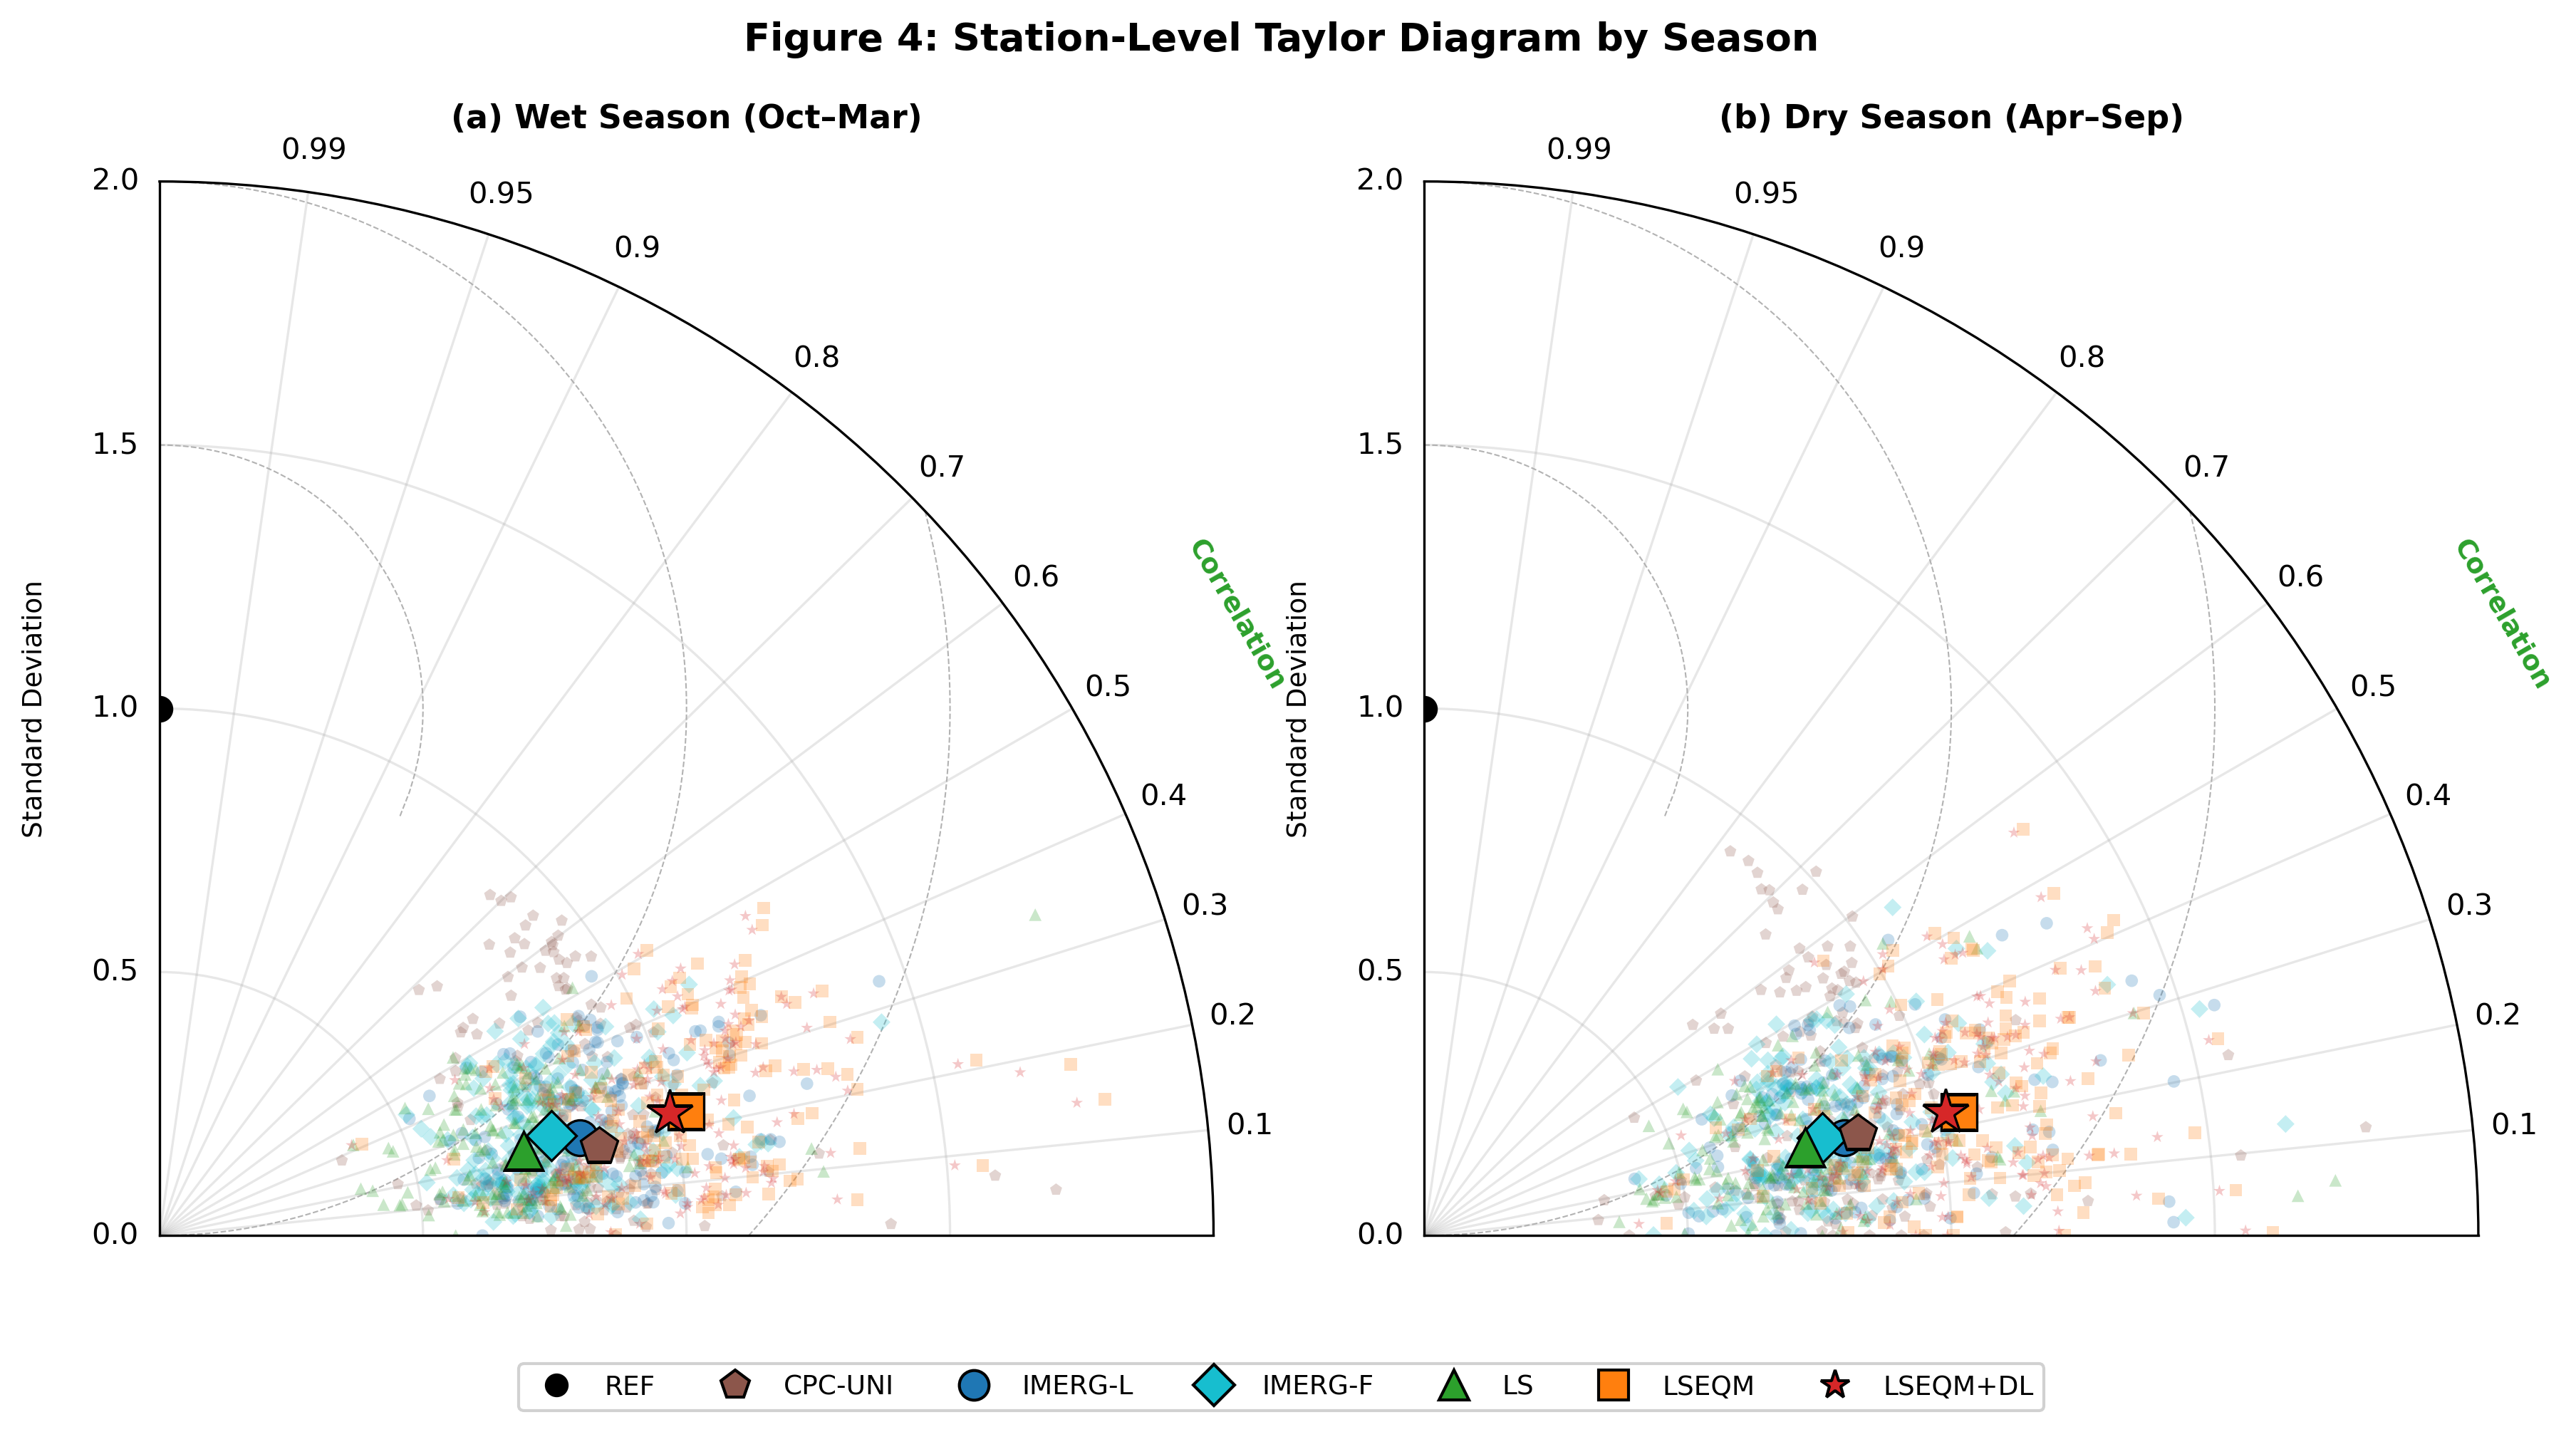
\includegraphics[width=\textwidth]{images/fig04_taylor_by_station.png}
\caption{Taylor diagrams comparing daily precipitation performance against independent BMKG station observations, stratified by (a) wet season (October--March) and (b) dry season (April--September). Products shown: CPC-UNI (brown pentagon), IMERG-L (blue circle), IMERG-F (cyan diamond, included as an independent benchmark), LS (green triangle), LSEQM (orange square), and LSEQM+DL (red star). Large markers indicate the median of per-station normalized statistics; small translucent markers show individual stations. The black circle at correlation = 1.0 and normalized standard deviation = 1.0 represents the station reference. Angular position indicates Pearson correlation, radial distance indicates normalized standard deviation, and gray dashed arcs indicate centered RMSE \cite{ref35}. Statistics are computed from daily paired values across all dekadal periods within each season, for stations with \(\geq\) 30 valid observation days.\label{fig4}}
\end{figure}

The domain-wide averages in \hyperref[tab:3]{Table~3} aggregate regions where the CPC-UNI
reference is well constrained by gauge observations alongside
station-sparse areas where CPC-UNI itself carries substantial
interpolation uncertainty. To disentangle this effect, the analysis was
stratified using the station density confidence mask (\hyperref[role-station-density]{Section~3.6}). In
station-covered regions (confidence \(C \geq 0.5\), 59 land pixels concentrated in densely gauged areas of Java and parts of Sumatra; this small footprint reflects Indonesia's actual gauge geography rather than a methodological choice), the CNN refinement effect is clearly
visible: the standard deviation ratio improves from 1.16 (LSEQM) to 1.05
(LSEQM+DL), and RMSE decreases from 9.0 to 8.3 mm/day. The relative bias
drops from 0.050 (LSEQM) to 0.003 (LSEQM+DL), confirming that the CNN is
most effective where the CPC-UNI reference is well constrained. In
station-sparse regions (\(C < 0.5\)), the LSEQM-to-LSEQM+DL transition
is minimal, reflecting the confidence mask design that reverts toward
purely statistical corrections where few gauges constrain the analysis.
This spatial dependence is explored further in \hyperref[role-station-density]{Section~3.6}.

A per-pixel quantile decomposition of the residual bias (Supplementary S4) reveals that IMERG is systematically too wet on CPC-UNI light-rain days and too dry on moderate-to-heavy days, a conditional mismatch that univariate quantile mapping cannot remove by construction \cite{ref34,ref11}. This structure explains the persistence of residual bias after LSEQM correction and is discussed further in the context of residual bias attribution (\hyperref[discussion]{Section~3.8}).

\subsection{Spatial Distribution of Correction
Quality}\label{spatial-distribution}

\hyperref[fig5]{Figure~5} presents the climatological mean daily precipitation for January dekad 1 (peak monsoon) across the IMERG products, the CPC-UNI reference, and the three correction stages. The wet bias of IMERG-L over interior Sumatra and Borneo is visibly reduced after LS and further refined by LSEQM, with the LSEQM+DL field most closely matching the reference pattern. This visual progression complements the metric-based assessment that follows.

\begin{figure}[H]
\centering
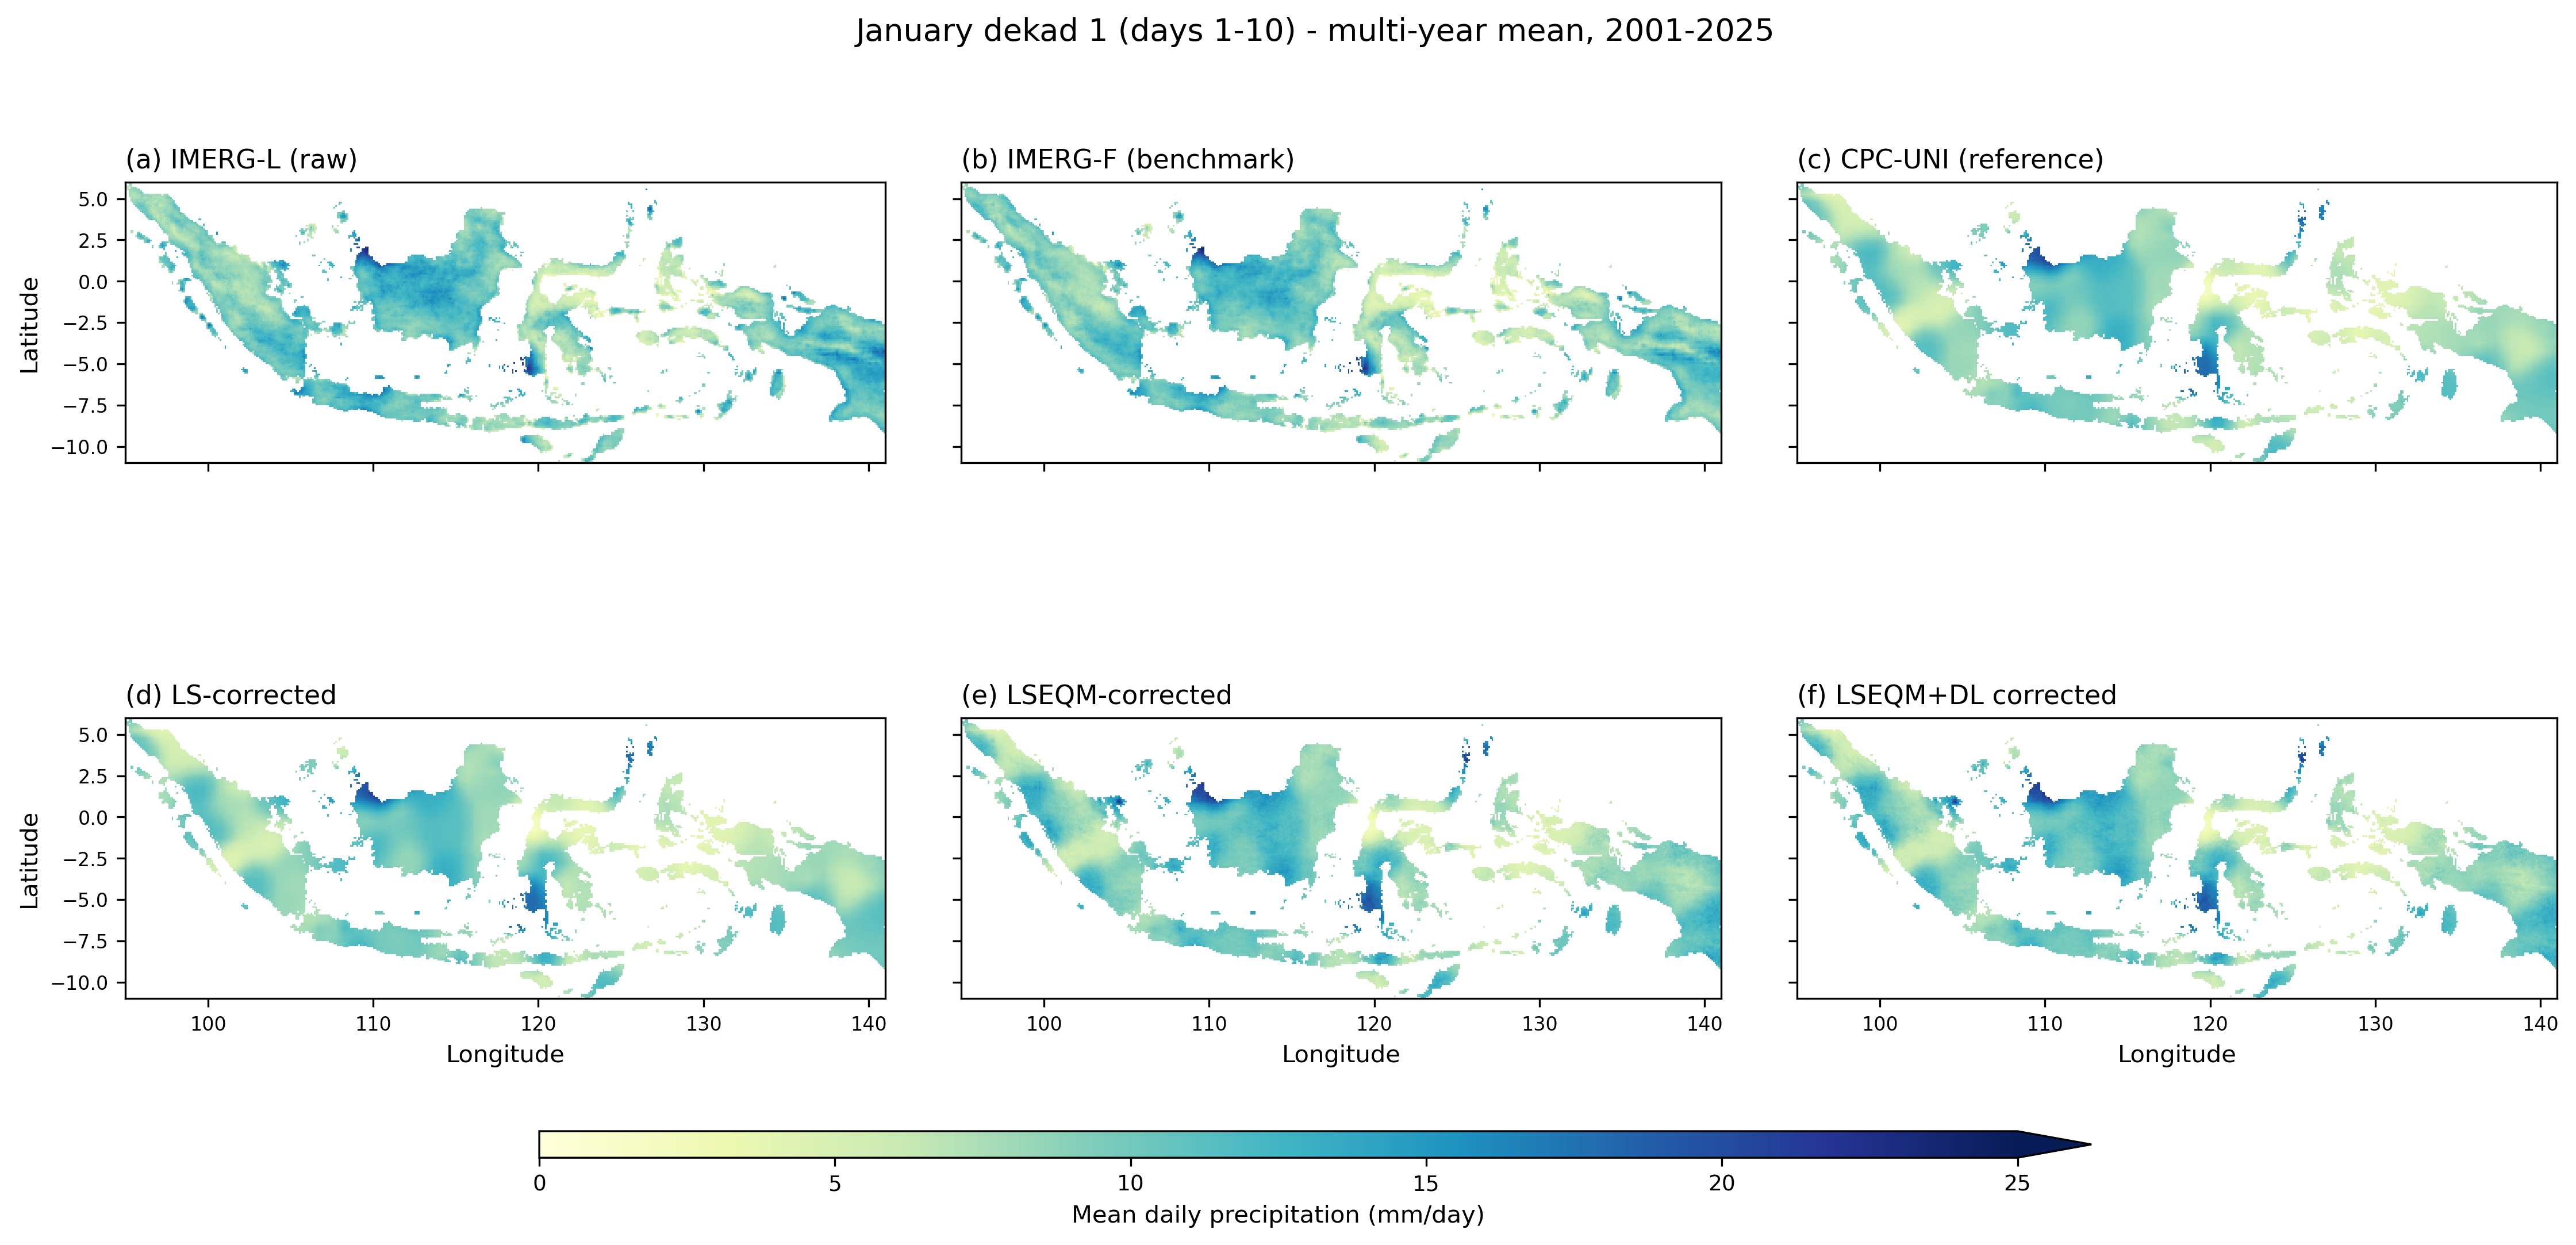
\includegraphics[width=\textwidth]{images/fig_compilation_jan_d1_mean_2001_2025.png}
\caption{Climatological mean daily precipitation (mm/day) for January dekad 1 (days 1--10), averaged over 2001--2025: (a) IMERG-L (raw satellite product to be corrected), (b) IMERG-F (gauge-adjusted satellite benchmark), (c) CPC-UNI (gauge-based reference at \(0.5^{\circ}\), regridded to \(0.1^{\circ}\)), (d) LS-corrected, (e) LSEQM-corrected, (f) LSEQM+DL corrected. All panels use a common color scale; ocean cells are masked. The progression from (a) to (f) visualizes the framework's effect on spatial precipitation patterns over the Indonesian archipelago.\label{fig5}}
\end{figure}

While domain-averaged statistics provide a useful summary, they mask
important spatial heterogeneity in correction performance. \hyperref[fig6]{Figure~6}
presents the Continuous Quality Index (CQI) spatial maps for all three
correction stages, computed as the mean CQI across all 36 dekadal
periods to provide a climatological summary of correction quality.

The CQI maps reveal a clear west-to-east gradient in correction quality.
Java, southern Sumatra, and Bali, regions characterized by dense gauge
networks and relatively homogeneous terrain at the CPC-UNI resolution,
consistently achieve CQI values in the Fair to Good range (0.5--0.65)
across all three methods. Eastern Indonesia, including Papua and Maluku,
shows lower CQI values, reflecting both the sparser station coverage of
the CPC-UNI reference and the greater topographic complexity of these
regions. The CQI ranges are {[}0.337, 0.657{]} for LS, {[}0.283,
0.602{]} for LSEQM, and {[}0.285, 0.608{]} for LSEQM+DL.

The domain-median CQI decreases from 0.541 (LS) to 0.505 (LSEQM) and
recovers slightly to 0.508 (LSEQM+DL). This decrease may appear to
contradict the distributional improvements documented in \hyperref[progressive-improvement]{Section~3.1},
but it reflects the composite nature of CQI: the Temporal Quality Score
(TQS), which includes POD and CSI, decreases from 0.666 to 0.648 because
the dry-day frequency matching \cite{ref11} reclassifies some IMERG wet days
as dry (reducing POD from 0.77 to 0.71), while the Basic Statistical
Quality Score (BSQS) decreases from 0.326 to 0.297 (LSEQM) and 0.299
(LSEQM+DL) due to the increase in RMSE that accompanies the wider
corrected distribution. These losses outweigh the gains in Distribution
Quality Score (DQS: 0.686 to 0.656 for LSEQM, recovering to 0.661 for
LSEQM+DL). The CNN refinement partially recovers performance (LSEQM+DL
CQI 0.508 vs LSEQM 0.505), consistent with the targeted spatial
adjustment in station-covered regions.

\begin{figure}[H]
\centering
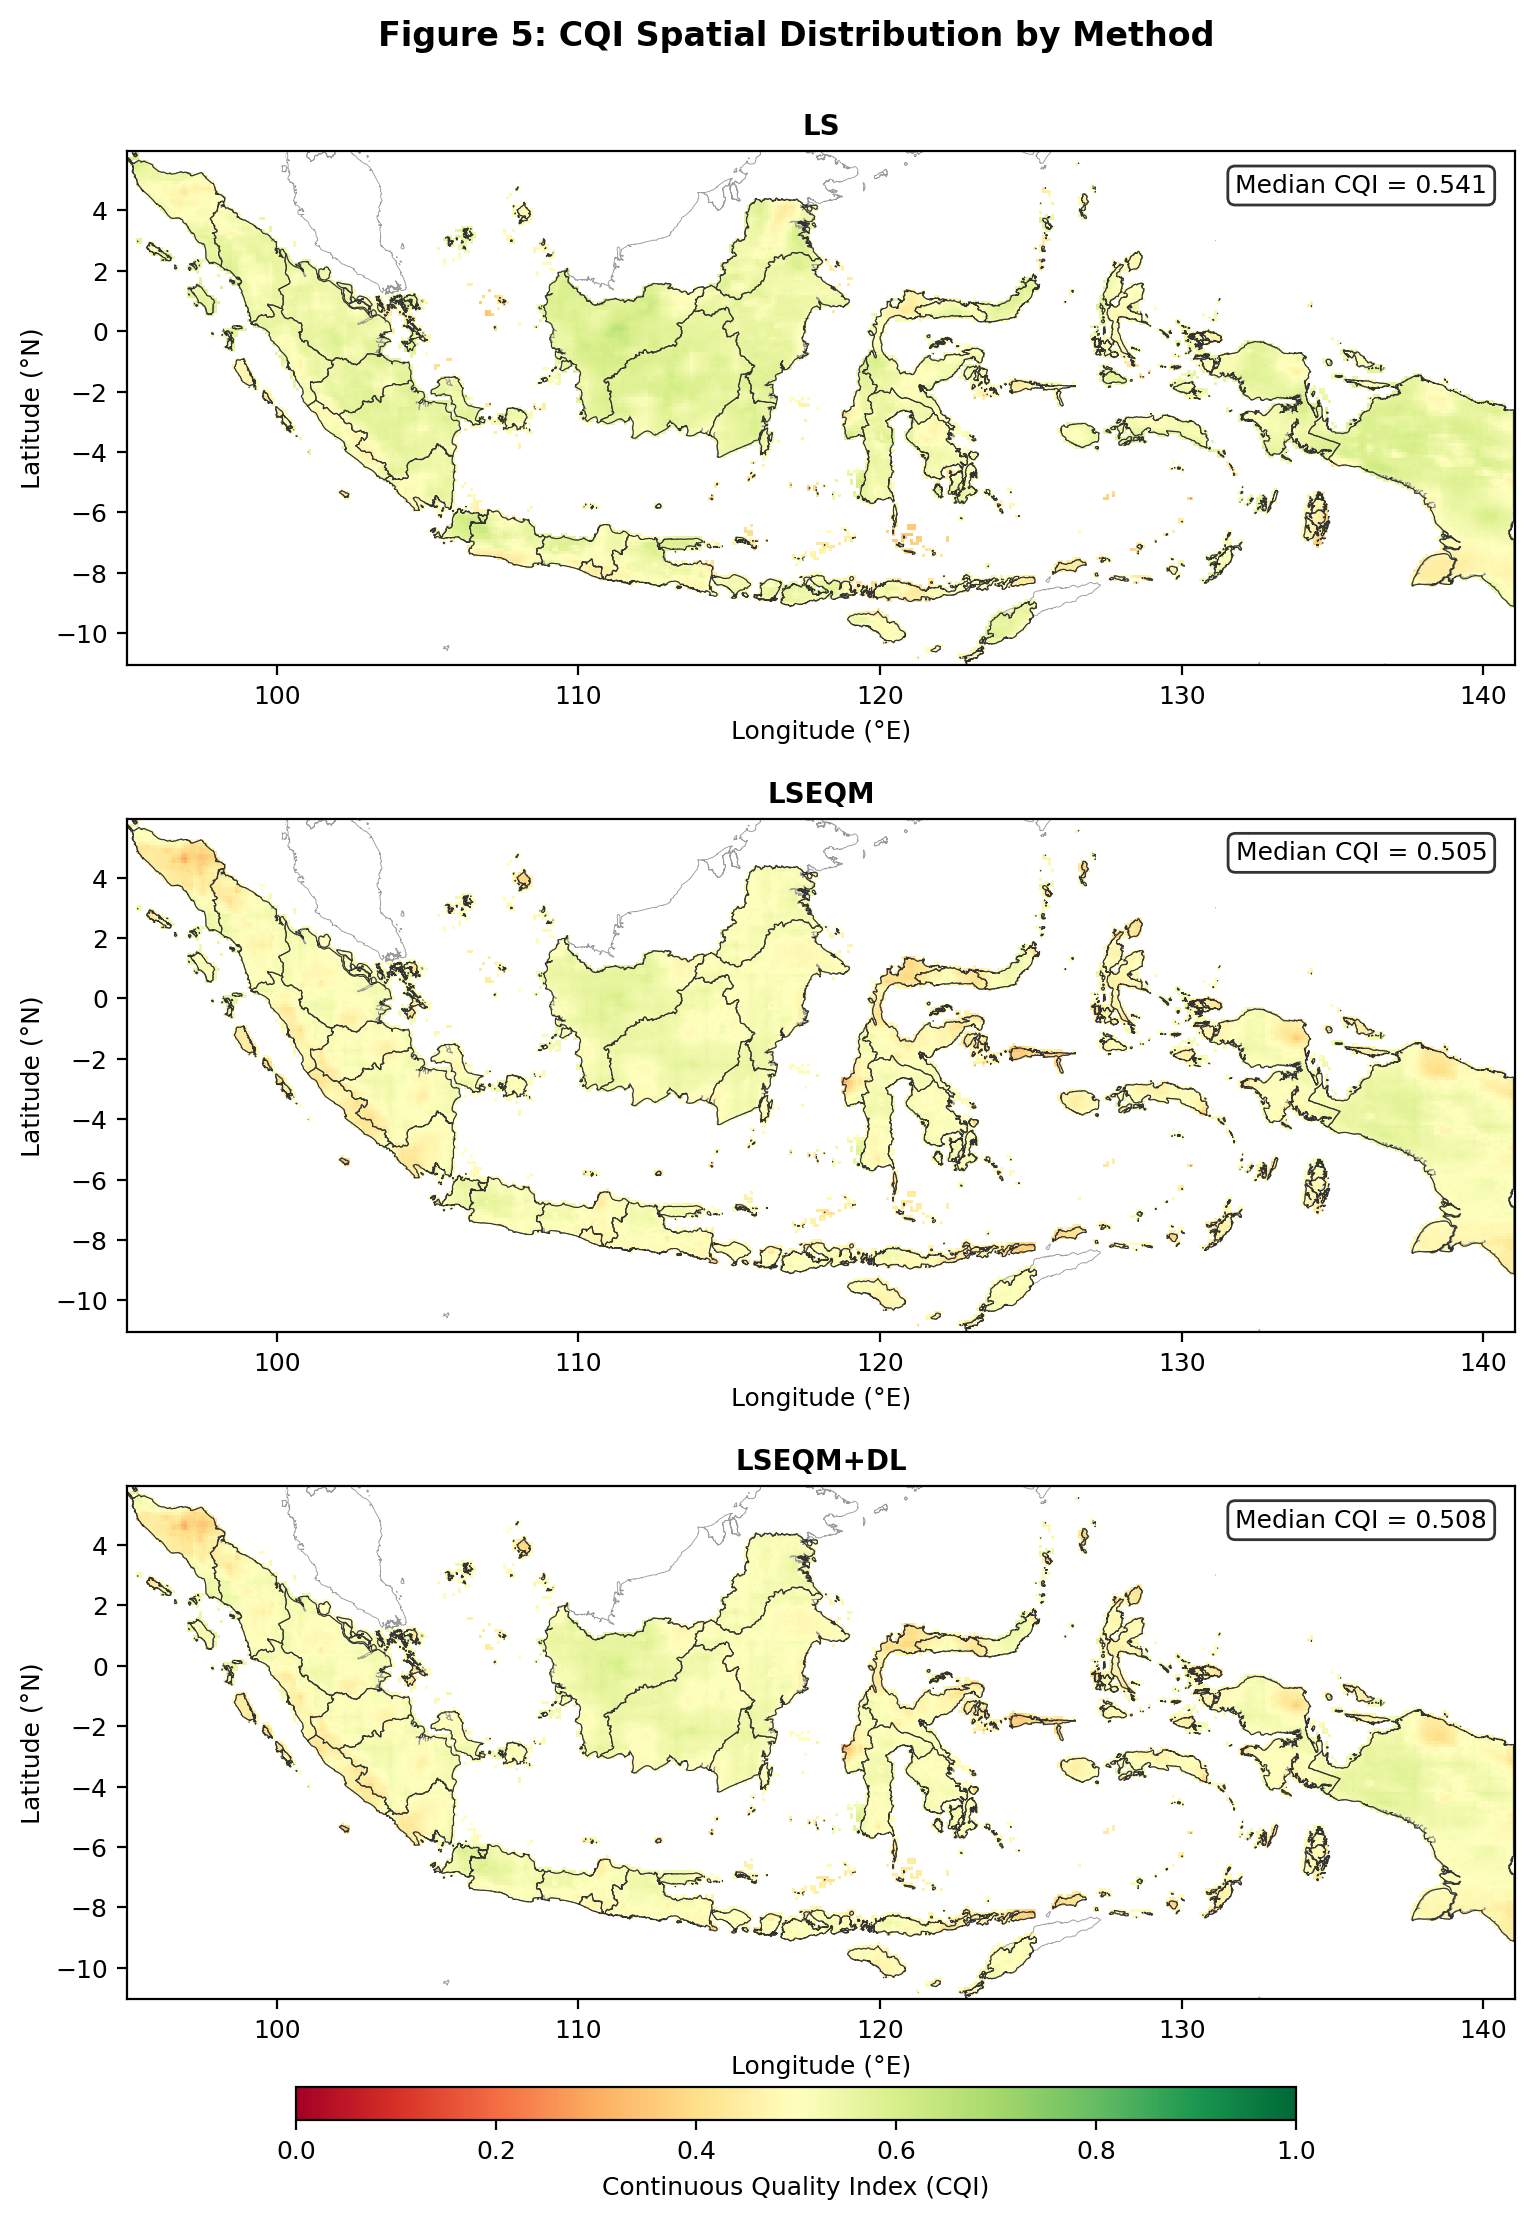
\includegraphics[width=\textwidth]{images/fig05_cqi_spatial.png}
\caption{Spatial distribution of the Continuous Quality Index (CQI) for (a) Linear Scaling, (b) LSEQM, and (c) LSEQM+DL, evaluated against CPC-UNI. Values represent the mean CQI across all 36 dekadal periods. Higher values indicate better agreement with the reference dataset. The color scale ranges from 0 (poor) to 1 (excellent).}\label{fig6}
\end{figure}

\hyperref[fig7]{Figure~7a} presents a smoothed CQI difference map (LSEQM+DL minus LS),
showing a spatially heterogeneous pattern: regions with higher station
density (Java, Bali, southern Sumatra) tend to show modest CQI gains
from the CNN refinement, while the domain majority shows small decreases
driven by the POD/RMSE trade-off discussed above. \hyperref[fig7]{Figure~7b} presents a
six-tier quality classification for LSEQM+DL that subdivides the
dominant Fair range (0.4--0.6) to reveal spatial structure: the majority
of land pixels fall in the Fair-High (0.5--0.6) and Fair-Low (0.4--0.5)
categories, with a clear west-to-east gradient from Fair-High in
station-dense regions to Fair-Low and Marginal (0.3--0.4) in
station-sparse eastern Indonesia. Only 2 pixels reach Good (\(\geq\)
0.6); no pixels achieve Excellent (\(\geq\) 0.7).

\begin{figure}[H]
\centering
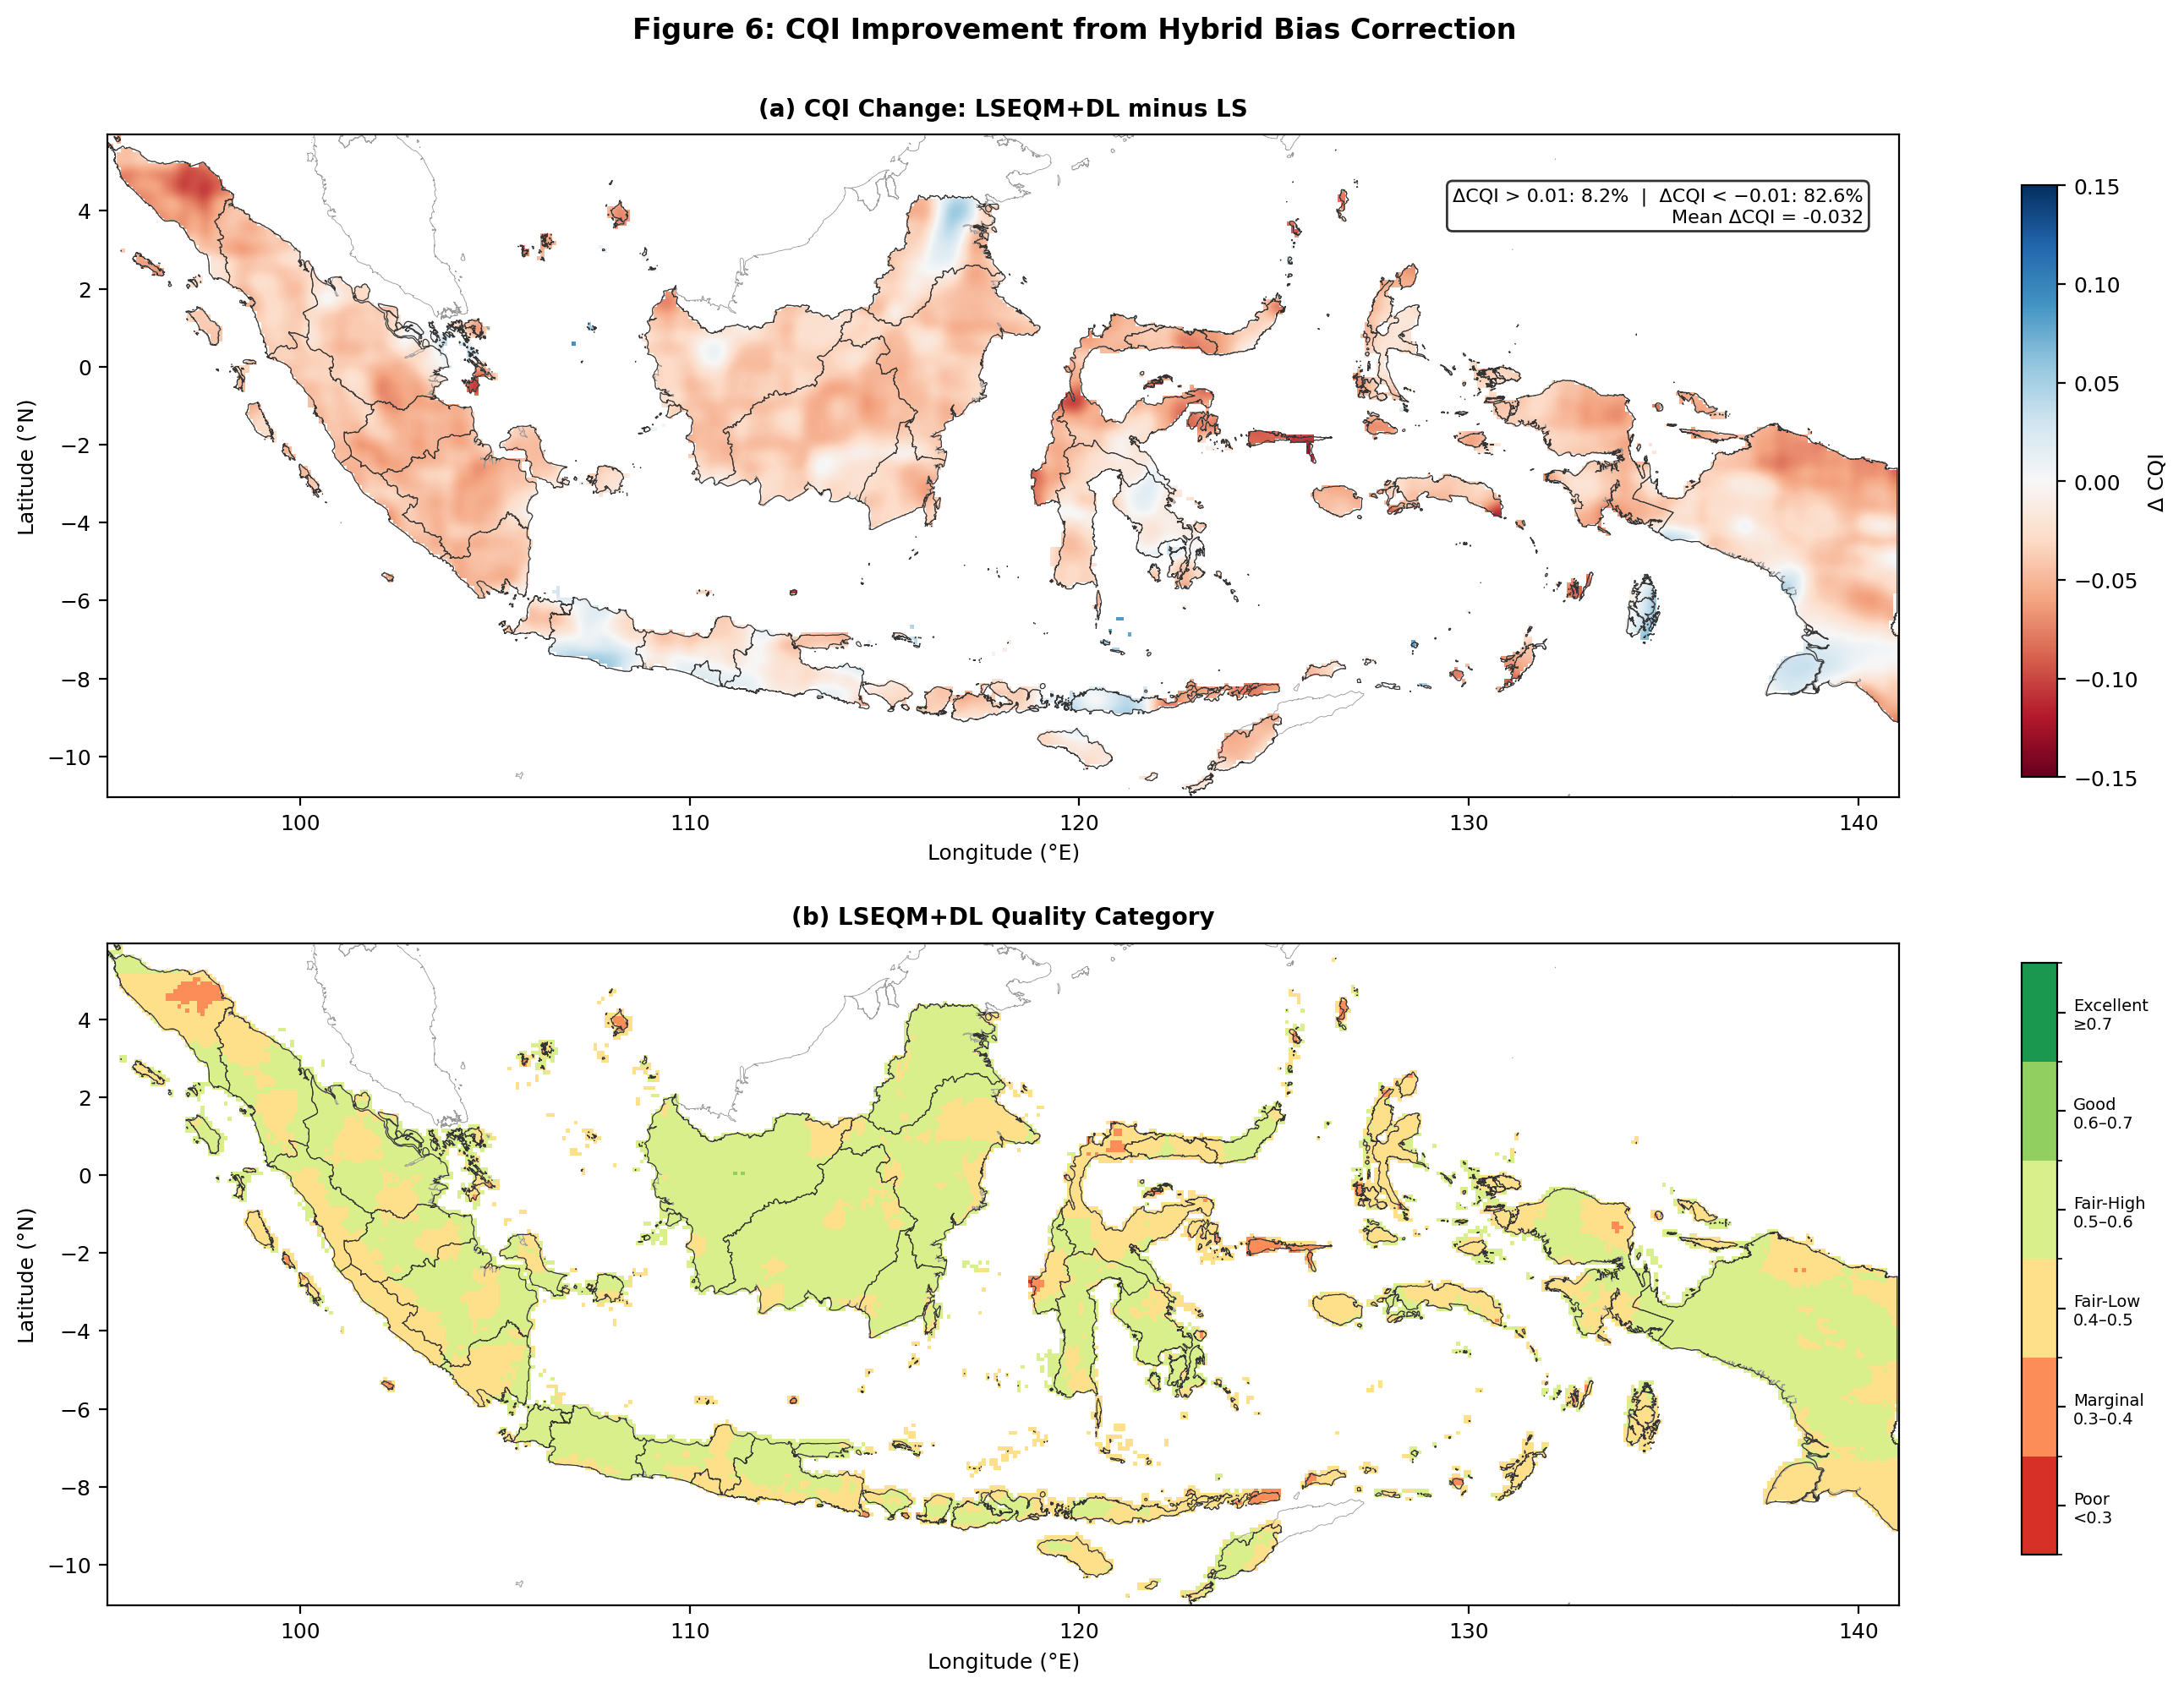
\includegraphics[width=\textwidth]{images/fig06_cqi_improvement.png}
\caption{(a) Smoothed CQI difference map showing the mean difference between LSEQM+DL and LS across all 36 dekadal periods (positive values indicate improvement; Gaussian smoothing with \(\sigma = 1.5\) pixels applied for visual clarity). (b) Six-tier quality classification of LSEQM+DL: Excellent (\(\geq\) 0.7, dark green), Good (0.6--0.7, green), Fair-High (0.5--0.6, yellow-green), Fair-Low (0.4--0.5, yellow), Marginal (0.3--0.4, orange), and Poor (\textless{} 0.3, red).}\label{fig7}
\end{figure}

The spatial pattern of the CQI difference correlates with station
density, a relationship explored further in \hyperref[role-station-density]{Section~3.6}. The CNN
refinement shows its largest positive contribution in station-dense
regions, indicating that the alpha-blending strategy and station density
confidence mask effectively target the DL contribution where the
reference is well constrained. This CQI result highlights an important
methodological point: composite quality indices that weight event
detection equally with distributional accuracy may undervalue
corrections that deliberately trade wet-day frequency for distributional
fidelity. The independent station validation (\hyperref[station-level-ground-truth-validation]{Section~3.5}) provides the
clearest assessment of the framework's net benefit.

\subsection{Distributional Quality and Extreme Event
Representation}\label{distributional-quality}

A central motivation for the hybrid framework is the preservation of
extreme precipitation events \cite{ref46}, which are often attenuated by
standard bias correction methods. \hyperref[tab:4]{Table~4} presents the domain-median
percentile values for the CPC-UNI reference and each correction stage,
spanning from the median (Q50) to the 99th percentile (Q99). Percentiles
are computed from the single-dekad aggregated mode, which pools
approximately 230 daily values per pixel (25 years \(\times\) 10 days
per dekad on average, with the actual count varying by dekad length and missing days), providing adequate sample sizes for stable quantile
estimation.

\phantomsection\label{tab:4}
\textbf{Table 4.} Domain-median precipitation percentiles (mm/day) for
the CPC-UNI reference and each correction stage, averaged over all 36
dekadal periods. Values in parentheses indicate the relative error
against the reference.

\begingroup\small
\begin{longtable}[]{@{}lllll@{}}
\toprule
Percentile & CPC-UNI & LS, \% Err & LSEQM, \% Err & LSEQM+DL, \% Err \\
\midrule
\endhead
\bottomrule
\endlastfoot
\(Q_{25}\) & 0.27 & 0.44 (+62.6\%) & 0.00 ($-$100\%) & 0.00 ($-$100\%) \\
\(Q_{50}\) & 2.22 & 2.62 (+18.0\%) & 1.71 ($-$23.1\%) & 1.71 ($-$23.1\%) \\
\(Q_{75}\) & 8.64 & 8.84 (+2.4\%) & 8.76 (+1.4\%) & 8.76 (+1.4\%) \\
\(Q_{90}\) & 20.22 & 19.47 ($-$3.7\%) & 22.67 (+12.1\%) & 22.61 (+11.8\%) \\
\(Q_{95}\) & 29.80 & 28.47 ($-$4.5\%) & 35.53 (+19.2\%) & 35.27 (+18.4\%) \\
\(Q_{99}\) & 51.31 & 50.59 ($-$1.4\%) & 63.19 (+23.2\%) & 62.46 (+21.7\%) \\
\end{longtable}
\endgroup

LS preserves the relative percentile structure through uniform multiplicative rescaling; the small apparent errors at \(Q_{90}\) and above against CPC-UNI are a statistical coincidence arising from cancellation of wet-day intensity under-prediction and frequency over-prediction. The LSEQM stage shifts the upper percentiles upward through gamma-based quantile mapping and explicit dry-day handling. Crucially, at independent BMKG stations (\hyperref[station-level-ground-truth-validation]{Section~3.5}), the \(Q_{99}\) ratio moves from 0.71 (LS) to 1.01 (LSEQM+DL): the shift away from CPC-UNI is a shift \emph{toward} gauge ground truth.

\hyperref[fig8]{Figure~8} presents the distribution of CQI component scores across all
land pixels, comparing the three correction stages. The box plots reveal
that all three CQI components decrease from LS to LSEQM, with partial
recovery under LSEQM+DL. The BSQS (median: LS 0.326, LSEQM 0.297,
LSEQM+DL 0.299) decreases because the wider corrected distribution
increases RMSE. The DQS (median: LS 0.686, LSEQM 0.656, LSEQM+DL 0.661)
decreases because the CPC-UNI-referenced KS statistic penalizes the
intentional distributional shift toward gauge ground truth. The TQS
(median: LS 0.666, LSEQM 0.648, LSEQM+DL 0.648) decreases because POD
and CSI drop as the dry-day handling \cite{ref11} reclassifies some IMERG
wet days. These component-level patterns explain the overall CQI
decrease discussed in \hyperref[spatial-distribution]{Section~3.2} and underscore the tension between
CPC-UNI-referenced composite indices and the independent station
validation (\hyperref[station-level-ground-truth-validation]{Section~3.5}), which confirms that the distributional
corrections represent genuine improvements.

\begin{figure}[H]
\centering
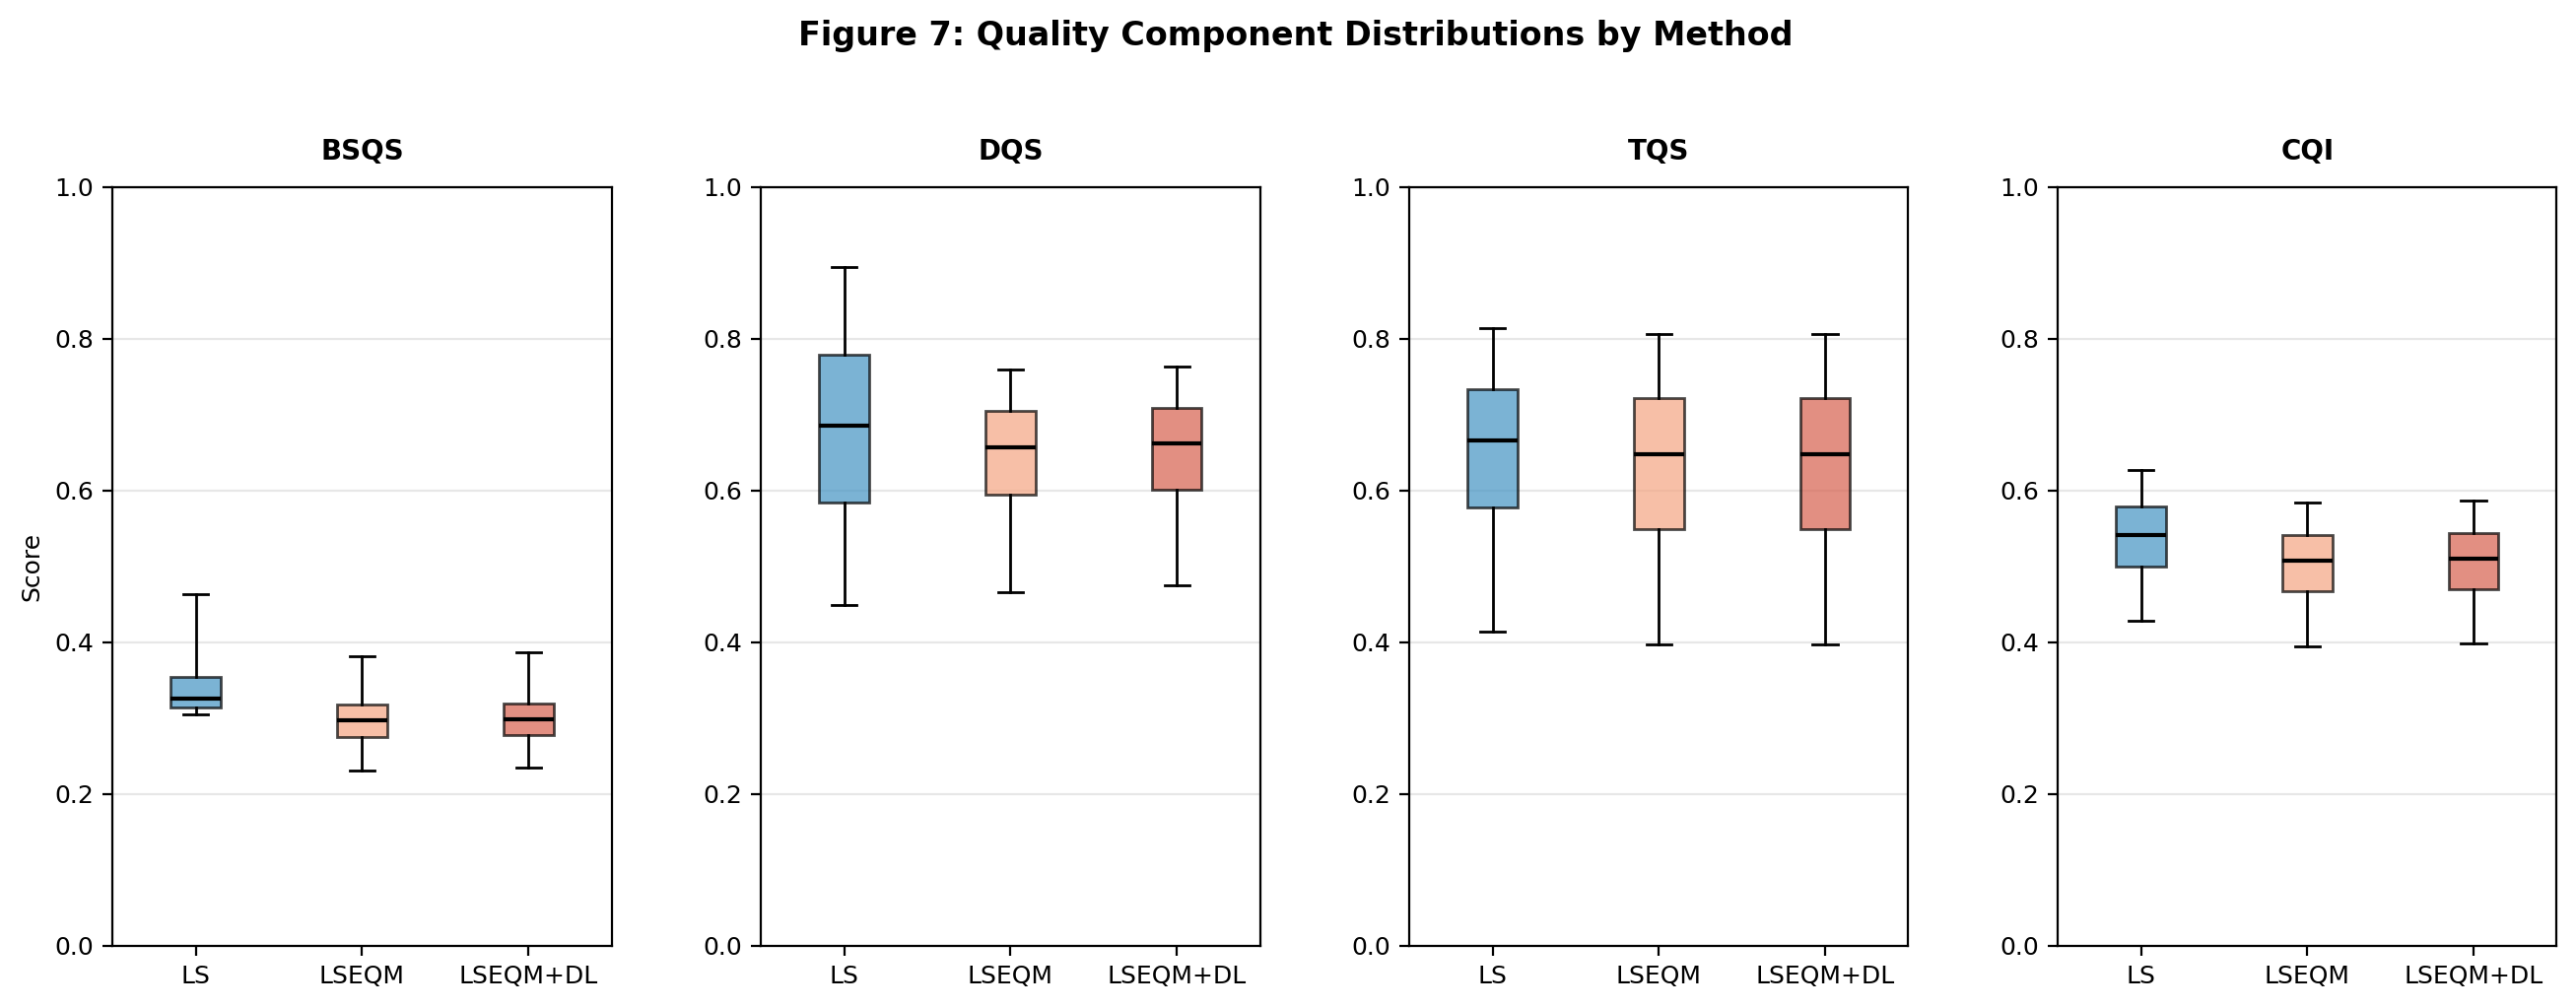
\includegraphics[width=\textwidth]{images/fig07_component_boxplots.png}
\caption{Distribution of CQI component scores across all land pixels for LS (blue), LSEQM (orange), and LSEQM+DL (green): (a) Basic Statistical Quality Score (BSQS), (b) Distribution Quality Score (DQS), (c) Temporal Quality Score (TQS), and (d) overall Continuous Quality Index (CQI). Box plots show the median, interquartile range, and 5th--95th percentile whiskers.}\label{fig8}
\end{figure}

The KS \(p\)-value against CPC-UNI decreases from 6.56\% (LS) to 0.00\% (LSEQM), but at independent BMKG stations it improves from 0.01\% to 19.07\%, confirming that the intentional distributional shift represents genuine improvement against uncontaminated ground truth. The LSEQM+DL value (also 19.07\%, Table~6) is identical to LSEQM at this precision, since CNN refinement modifies values only at pixels exceeding the 80th LSEQM percentile and leaves the bulk of the marginal distribution unchanged.

\subsection{Cross-Reference
Evaluation}\label{cross-reference-evaluation}

Evaluating bias-corrected products solely against the training reference
(CPC-UNI) risks overly optimistic performance estimates. The evaluation
framework includes cross-reference validation against both the IMERG
Final Run (IMERG-F), a gauge-adjusted satellite product not used in the
correction procedure (\hyperref[nine-combination-evaluation-design]{Section~2.4.1}), and the uncorrected IMERG Late Run
(IMERG-L) as a baseline. This implements the 3 \(\times\) 3 factorial
design described in \hyperref[tab:1]{Table~1}, enabling three complementary evaluation
perspectives. IMERG-F is also included in the station-level Taylor
diagram (\hyperref[fig4]{Figure~4}) as an independent benchmark.

\hyperref[tab:5]{Table~5} presents the full evaluation matrix using metrics aligned with
the three-pillar framework. Metrics are summarized as domain-wide
medians averaged over all 36 dekadal periods.

\phantomsection\label{tab:5}
\textbf{Table 5.} Cross-reference evaluation matrix organized by the
three-pillar framework. RB = Relative Bias (value adjustment), SDR =
Std. Dev. Ratio, KS \(p\) = Kolmogorov-Smirnov \(p\)-value (distribution
alignment), \(Q_{99}\)R = 99th-percentile ratio (extreme preservation),
CSI = Critical Success Index (event detection). Bold indicates the value
closest to target per reference group.

\begingroup\small
\begin{longtable}[]{@{}lllllll@{}}
\toprule
Reference & Test & RB & SDR & KS \(p\) (\%) & \(Q_{99}\) Ratio & CSI \\
\midrule
\endhead
\bottomrule
\endlastfoot
CPC-UNI & LS & \textbf{0.0000} & \textbf{0.9707} & \textbf{6.56} &
\textbf{0.9669} & \textbf{0.5890} \\
& LSEQM & 0.0697 & 1.1587 & 0.00 & 1.2117 & 0.5723 \\
& LSEQM+DL & 0.0652 & 1.1475 & 0.00 & 1.1964 & 0.5724 \\
IMERG-F & LS & $-$0.0819 & 0.9549 & \textbf{51.25} & 0.9527 & \textbf{0.9016} \\
& LSEQM & \textbf{$-$0.0093} & 1.1384 & 0.00 & 1.2053 & 0.8574 \\
& LSEQM+DL & $-$0.0140 & \textbf{1.1274} & 0.00 & \textbf{1.1902} & 0.8574 \\
IMERG-L & LS & $-$0.1010 & 0.8990 & \textbf{62.26} & 0.8990 & \textbf{0.9643} \\
& LSEQM & \textbf{$-$0.0279} & 1.0783 & 0.00 & 1.1425 & 0.9117 \\
& LSEQM+DL & $-$0.0326 & \textbf{1.0678} & 0.00 & \textbf{1.1280} & 0.9116 \\
\end{longtable}
\endgroup

Against CPC-UNI, LS appears closest to target for most metrics because it preserves the satellite's distributional shape. The IMERG-F rows provide an independent perspective: relative bias decreases from $-$0.082 (LS) to $-$0.009 (LSEQM), indicating that distributional correction brings the product closer to the gauge-adjusted satellite estimate. The standard deviation ratio against IMERG-F moves from 0.95 (LS) toward 1.13 (LSEQM+DL), overshooting IMERG-F variability and consistent with the interpretation that LSEQM pushes the distribution toward independent gauge ground truth (\hyperref[station-level-ground-truth-validation]{Section~3.5}). Across all three reference groups, the KS \(p\)-value drops to zero after EQM, reflecting the intentional distributional shift confirmed as beneficial by station validation.

\subsection{Station-Level Ground Truth
Validation}\label{station-level-ground-truth-validation}

The gridded evaluation in \hyperref[progressive-improvement]{Sections~3.1--3.4} assesses correction
performance against the CPC-UNI reference used during training. The most
rigorous test of the framework employs entirely independent ground
truth. The corrected products were compared against daily precipitation
observations from 171 BMKG (Indonesian Meteorological, Climatological,
and Geophysical Agency) weather stations, which were not used in any
stage of the bias correction procedure. A minimum of 30 valid
overlapping days per station follows WMO guidance for precipitation
verification sample sizes; results are robust to increasing this
threshold to 60 days (up to 169 stations retained per dekad).

\hyperref[fig9]{Figure~9} presents the spatial distribution of BMKG stations alongside
the per-station standard deviation ratio for the LSEQM+DL product, which
measures how well the corrected product reproduces the observed
precipitation variability at each gauge location.

\begin{figure}[H]
\centering
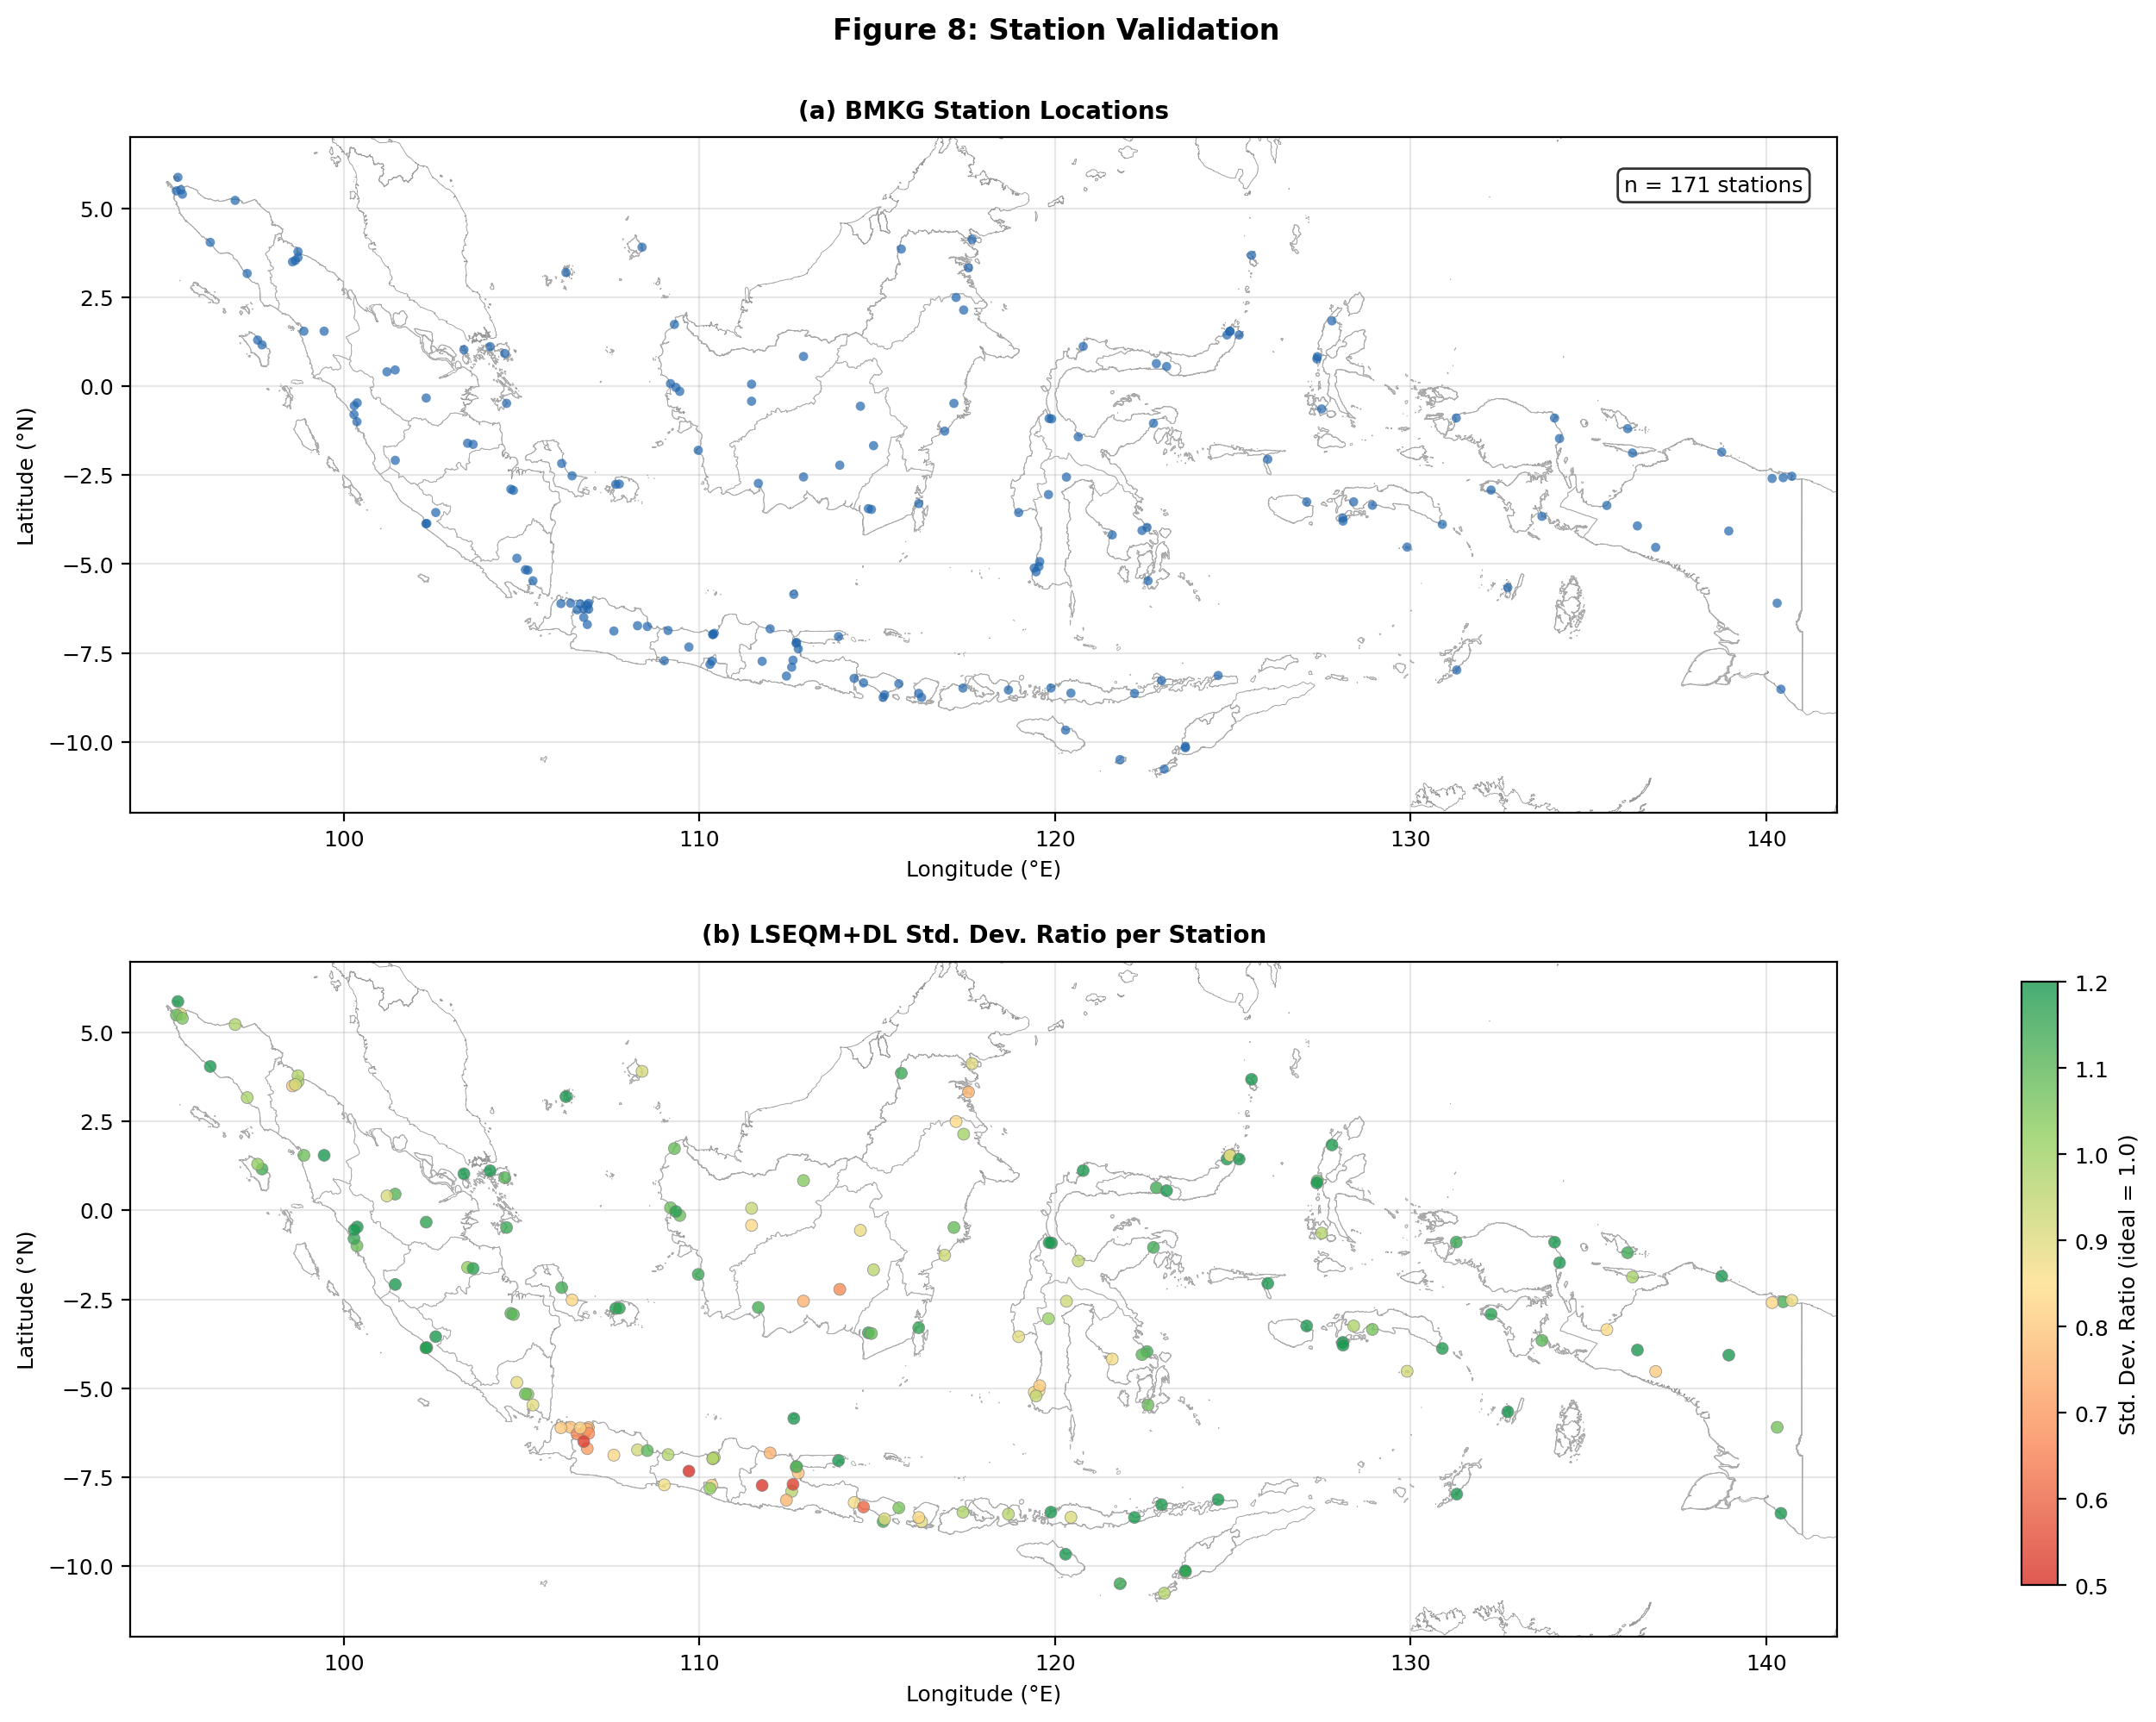
\includegraphics[width=\textwidth]{images/fig08_station_validation.png}
\caption{(a) Location of BMKG weather stations used for independent validation (\(n\) = 171). (b) Per-station standard deviation ratio (test/observed) for the LSEQM+DL product, averaged across all dekadal periods. Values near 1.0 (green) indicate good variability preservation; values below 0.7 (red) indicate underestimation of observed variability.}\label{fig9}
\end{figure}

\hyperref[tab:6]{Table~6} presents the station-level validation results organized by the
same three-pillar framework used for the domain-wide evaluation. The
station-level results provide the clearest evidence of the framework's
effectiveness, as the BMKG observations represent direct ground truth
uncontaminated by the interpolation uncertainties present in the gridded
CPC-UNI reference.

\phantomsection\label{tab:6}
\textbf{Table 6.} Independent station validation organized by the three
design objectives of the hybrid framework. Values represent the median
across 171 BMKG stations and all 36 dekadal periods. Ratio metrics
express test/observed (target = 1.0). Bold indicates the value closest
to the target.

\begingroup\small
\begin{longtable}[]{@{}llllll@{}}
\toprule
Evaluation Objective & Metric & LS & LSEQM & LSEQM+DL & Target \\
\midrule
\endhead
\bottomrule
\endlastfoot
\textbf{Value Adjustment} & Relative Bias & $-$0.114 & \textbf{0.009}
& $-$0.006 & 0 \\
& Std. Dev. Ratio & 0.71 & 1.03 & \textbf{1.00} & 1.0 \\
\textbf{Distribution Alignment} & KS \(p\)-value (\%) & 0.01 &
\textbf{19.07} & \textbf{19.07} & 100 \\
& Wet-Day Freq. Ratio & 1.21 & \textbf{0.96} & \textbf{0.95} & 1.0 \\
& Mean Wet-Day Precip Ratio & 0.71 & \textbf{1.06} & \textbf{1.05} &
1.0 \\
\textbf{Extreme Preservation} & \(Q_{95}\) Ratio & 0.74 & \textbf{1.07}
& \textbf{1.05} & 1.0 \\
& \(Q_{99}\) Ratio & 0.71 & 1.05 & \textbf{1.01} & 1.0 \\
\textbf{Event Detection} & POD & \textbf{0.78} & 0.65 & 0.65 & 1.0 \\
& CSI & \textbf{0.53} & 0.49 & 0.49 & 1.0 \\
& FAR & 0.36 & \textbf{0.32} & \textbf{0.32} & 0 \\
\end{longtable}
\endgroup

The station-level results provide strong evidence for the framework's
effectiveness at independent ground truth locations. The most striking
changes occur in the LS-to-LSEQM transition. For value adjustment, the
standard deviation ratio improves from 0.71 to 1.03, meaning that LS
underestimates the observed precipitation variability by 29\%, while
LSEQM matches it within 3\%. The LSEQM+DL standard deviation ratio
reaches 1.00 (exact match to observed variability). For distribution
alignment, the wet-day frequency ratio moves from 1.21 to 0.96,
correcting a 21\% overestimation of wet-day occurrence to within 5\% of
observed. For extreme preservation, the \(Q_{99}\) ratio improves from
0.71 to 1.05, recovering the large extreme rainfall underestimation
present in the LS product; the full LSEQM+DL reaches \(Q_{99}\) = 1.01
(near perfect). The mean wet-day precipitation ratio improves from 0.71
to 1.06, indicating that the EQM adjustment corrects a systematic 29\%
underestimation of rainfall intensity on wet days to within 6\% of
observed values.

These improvements come at a measurable cost in event detection: POD
decreases from 0.78 (LS) to 0.65 (LSEQM), while FAR improves from 0.36
to 0.32. This trade-off is inherent to the dry-day frequency matching
\cite{ref11} (\hyperref[hybrid-bias-correction-methodology]{Section~2.3}), which adjusts the marginal wet-day fraction to
match the CPC-UNI reference: some IMERG wet days that correspond to
genuine station-observed rainfall are reclassified as dry. However, the
net effect is that detected events are more reliable (lower FAR), and
the distributional properties of the corrected product are substantially
more accurate.

The LSEQM-to-LSEQM+DL transition shows targeted refinement at the
station level: the \(Q_{99}\) ratio moves from 1.05 to 1.01, and the
standard deviation ratio from 1.03 to 1.00, both approaching unity.
This confirms that the CNN refinement, while conservative by design,
provides measurable additional value for extreme event representation.

As with the gridded evaluation, temporal accuracy metrics at stations
show no improvement: Pearson correlation remains at approximately 0.24,
and RMSE increases from 15.9 (LS) to 18.2 mm/day (LSEQM+DL). This
confirms that the framework's value lies in statistical property
correction rather than temporal prediction skill, consistent with
\hyperref[progressive-improvement]{Section~3.1}.

To evaluate extreme event detection skill across a range of
precipitation intensities, the WMO-standard multi-threshold verification
\cite{ref24} was applied. \hyperref[fig10]{Figure~10} presents the Probability of Detection,
Critical Success Index, and Equitable Threat Score as functions of
precipitation threshold (1, 5, 10, 20, 50, 100, and 150 mm/day).

\begin{figure}[H]
\centering
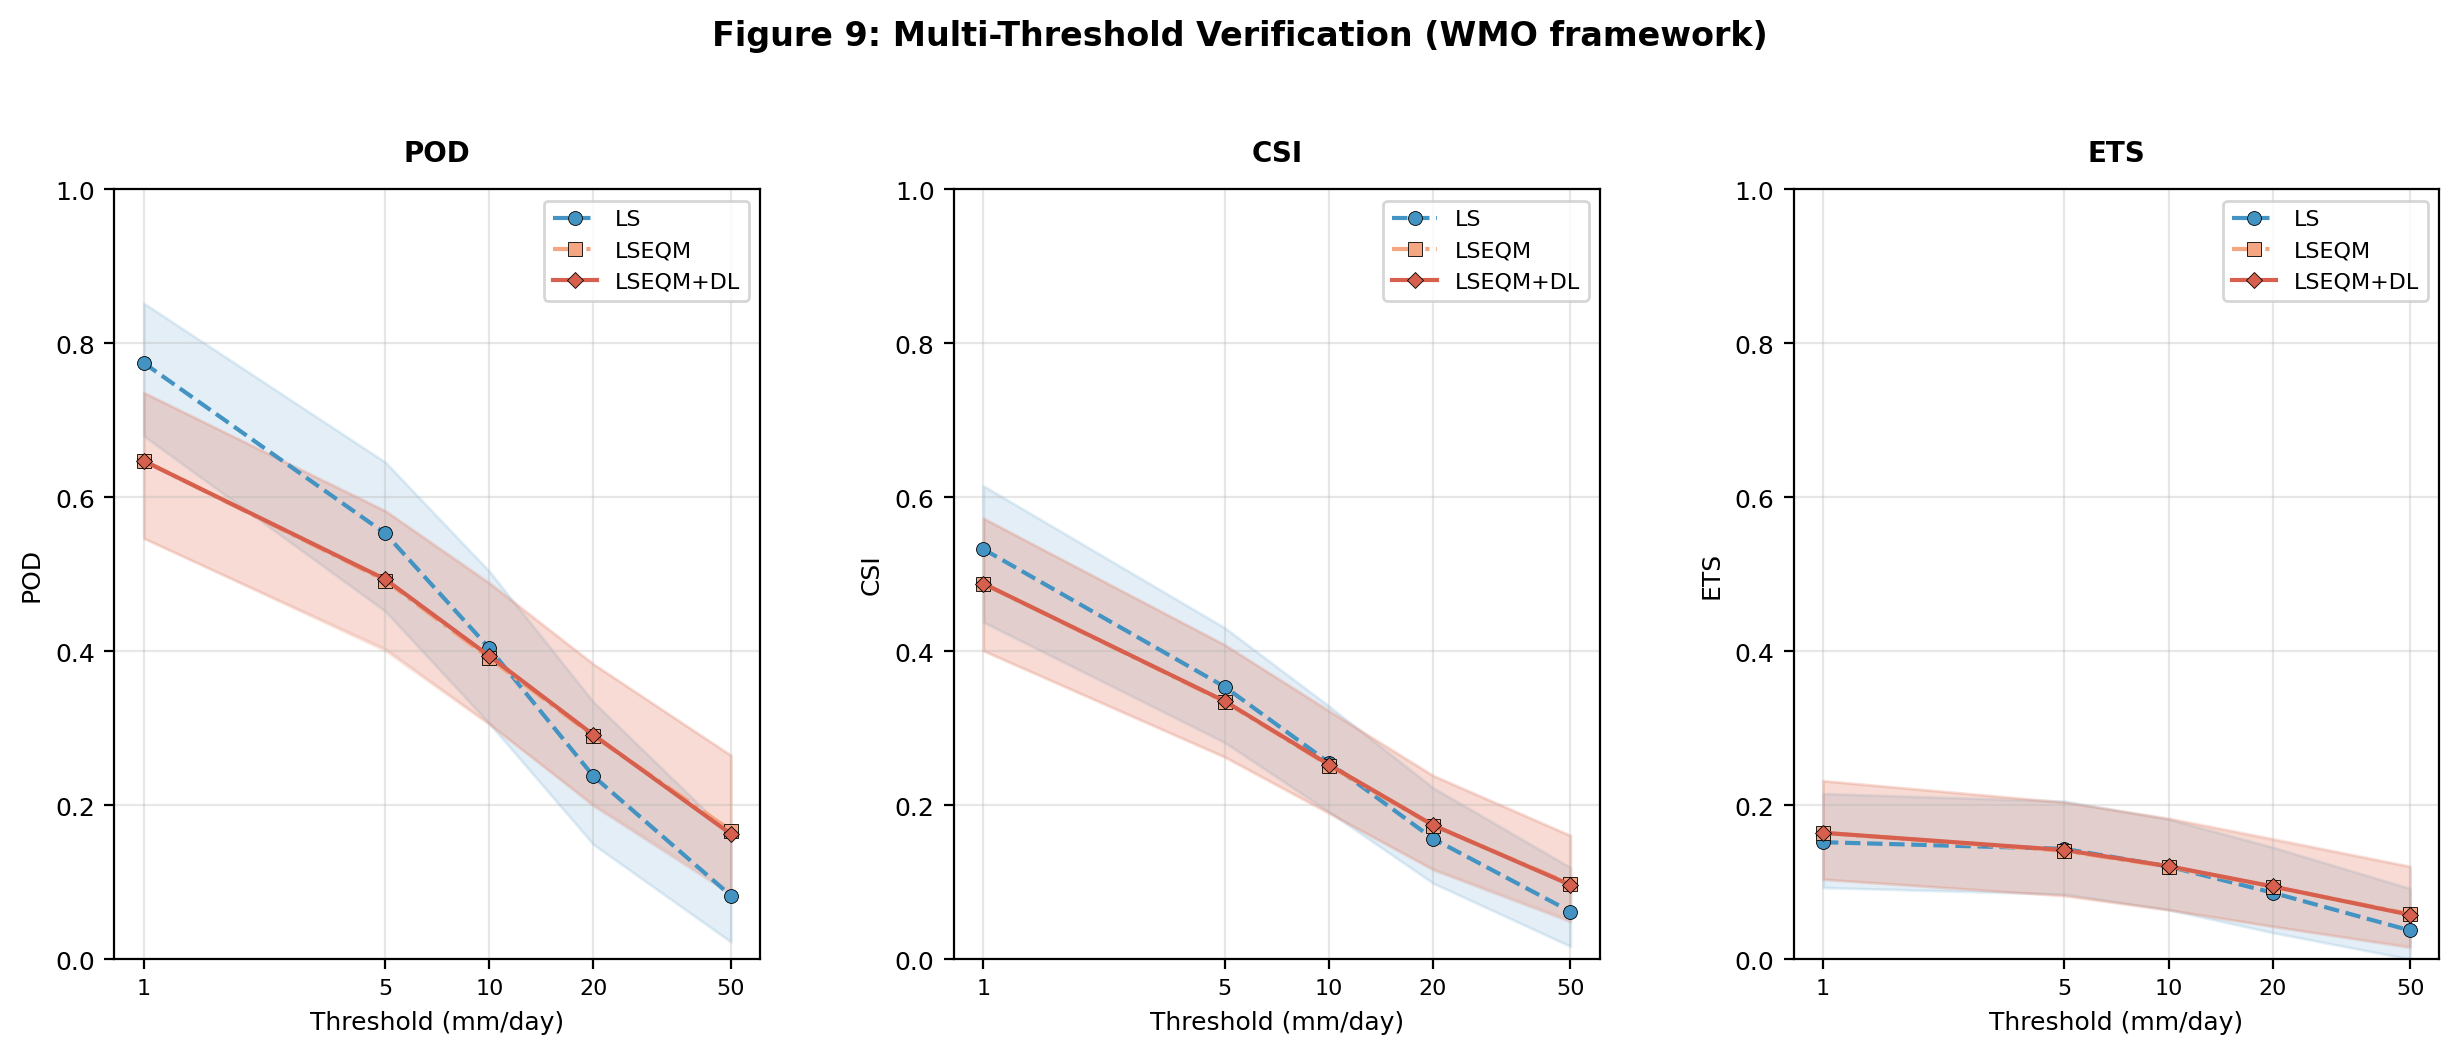
\includegraphics[width=\textwidth]{images/fig09_multi_threshold.png}
\caption{WMO multi-threshold verification: (a) Probability of Detection (POD), (b) Critical Success Index (CSI), and (c) Equitable Threat Score (ETS) as functions of precipitation threshold for LS (blue), LSEQM (orange), and LSEQM+DL (green). Lines show the median across all stations; shading indicates the interquartile range. Thresholds follow WMO classifications: 1 mm (measurable), 5 mm (light), 10 mm (moderate), 20 mm (moderate-heavy), 50 mm (heavy), 100 mm (very heavy), and 150 mm (extreme).}\label{fig10}
\end{figure}

All three methods show the expected decline in detection skill with
increasing threshold, as extreme events become rarer and more difficult
to reproduce. The LSEQM and LSEQM+DL curves are nearly indistinguishable
across all thresholds, reflecting the fact that the CNN refinement
adjusts precipitation magnitudes for extreme pixels but does not alter
wet/dry classification: the contingency tables underlying POD, CSI,
and ETS are therefore essentially identical for both methods. At the 1
mm threshold, LS achieves the highest POD (0.77) and CSI (0.53), while
LSEQM+DL shows lower POD (0.65) but also lower FAR, reflecting the
dry-day frequency matching \cite{ref11} described in \hyperref[hybrid-bias-correction-methodology]{Section~2.3}. However,
at thresholds above 20 mm/day, this pattern reverses: LSEQM and LSEQM+DL
maintain higher skill than LS. At the 50 mm threshold, the median CSI
for LSEQM+DL is 0.097, compared to 0.062 for LS, representing an
improvement of 56\%. At 100 mm (very heavy rainfall), the LSEQM+DL
product achieves a median POD of 0.065 and CSI of 0.042, compared to LS
values of 0.015 and 0.011 respectively. These absolute frequencies are
small because heavy-rainfall events are rare in the validation sample,
but the relative differences are consistent with the intended effect of
the GPD tail adjustment; statistical significance of the threshold-by-threshold
differences was not formally tested.
The Equitable Threat Score, which accounts for random hits, shows a
similar pattern: at 50 mm, the ETS for LSEQM+DL (0.058) exceeds that of
LS (0.038), confirming that the improved extreme detection is not
attributable to increased frequency bias.

These station-level results provide the strongest validation evidence in
this study, as BMKG observations are entirely independent of the
correction procedure and represent direct ground truth measurements.

\subsection{Role of the Station Density Confidence
Mask}\label{role-station-density}

The station density confidence mask was introduced to manage the spatial
heterogeneity of CPC-UNI reference quality by modulating the CNN
contribution based on gauge network density. To evaluate the
effectiveness of this mechanism, \hyperref[fig11]{Figure~11a} presents the confidence mask
itself, derived from BMKG station counts per CPC-UNI grid cell, and
\hyperref[fig11]{Figure~11b} examines the relationship between station density and CQI
improvement.

\begin{figure}[H]
\centering
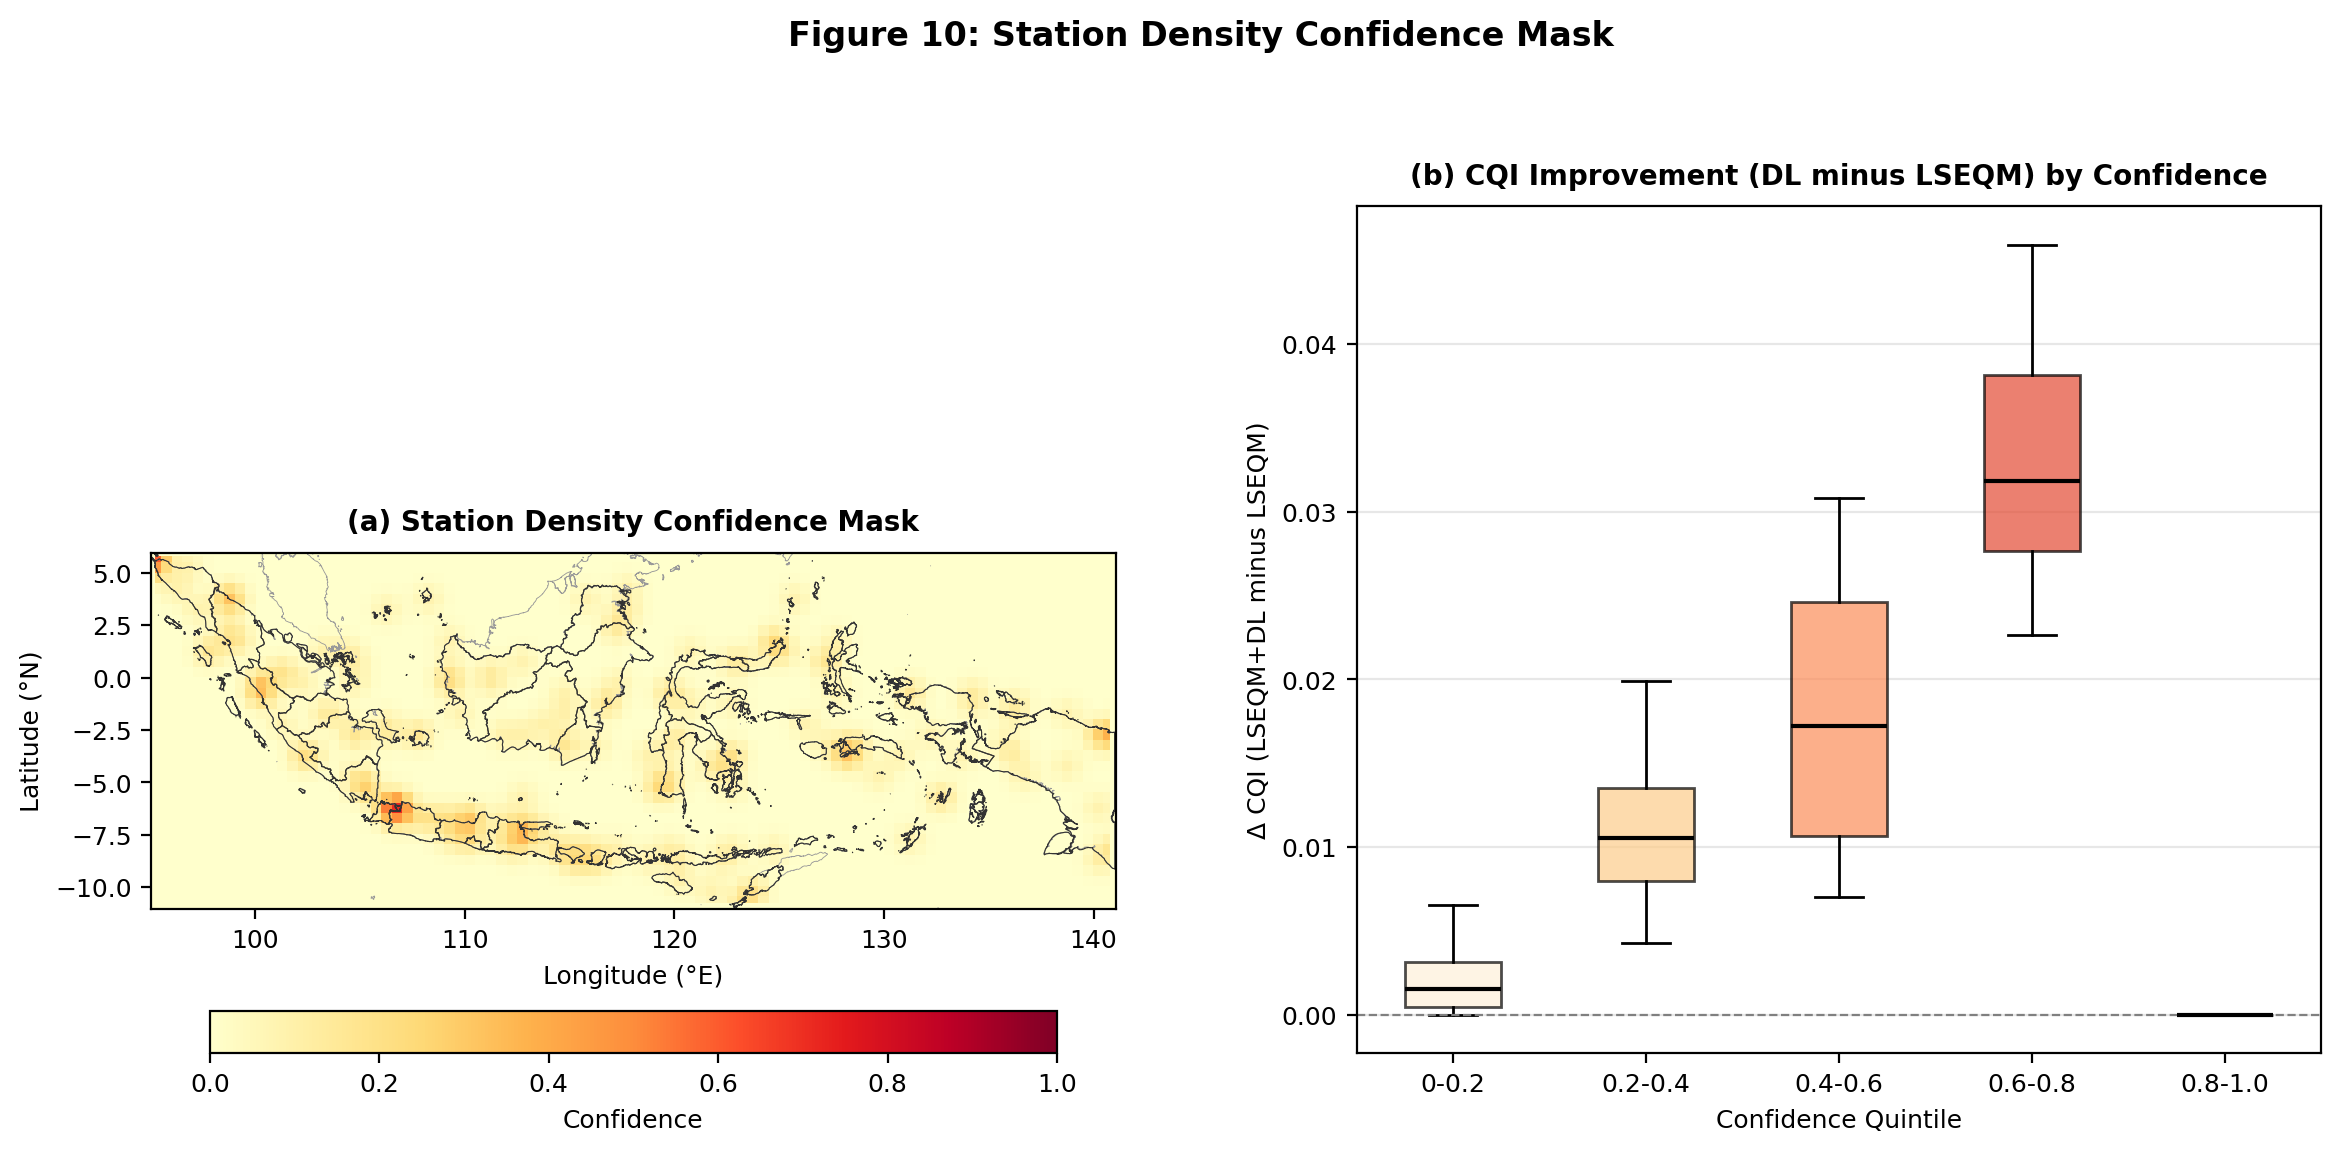
\includegraphics[width=\textwidth]{images/fig10_confidence_mask.png}
\caption{(a) Station density confidence mask \(C(x, y)\), ranging from 0 (no station coverage) to 1 (saturated coverage, \(\geq\) 2 stations per \(0.5^{\circ}\) cell). Gaussian smoothing (\(\sigma = 1\) grid cell) prevents sharp boundaries. (b) Relationship between confidence mask value and CQI improvement (LSEQM+DL minus LSEQM): box plots binned by confidence quintile.}\label{fig11}
\end{figure}

Java, Bali, and parts of Sumatra have high confidence (\(C > 0.7\)), while Papua, Maluku, and oceanic boundary regions have near-zero confidence (25.8\% of pixels have \(C = 0\)). The median \(\Delta\)CQI (LSEQM+DL minus LSEQM) increases monotonically with confidence, from +0.002 at \(C < 0.2\) to +0.032 at \(C \in [0.6, 0.8)\), confirming that the mask concentrates CNN refinement where the reference is well constrained and reverts to purely statistical corrections elsewhere. The mask also serves as a spatially explicit quality flag for operational agencies.

\subsection{Temporal Stability of
Corrections}\label{temporal-stability-of-corrections}

An important practical consideration for operational deployment is
whether the correction quality remains stable across the annual cycle or
varies systematically between wet and dry seasons. \hyperref[fig12]{Figure~12} presents
monthly domain-median values of four key metrics (standard deviation
ratio, RMSE, KS \(p\)-value, and CSI) for all three correction
stages.

\begin{figure}[H]
\centering
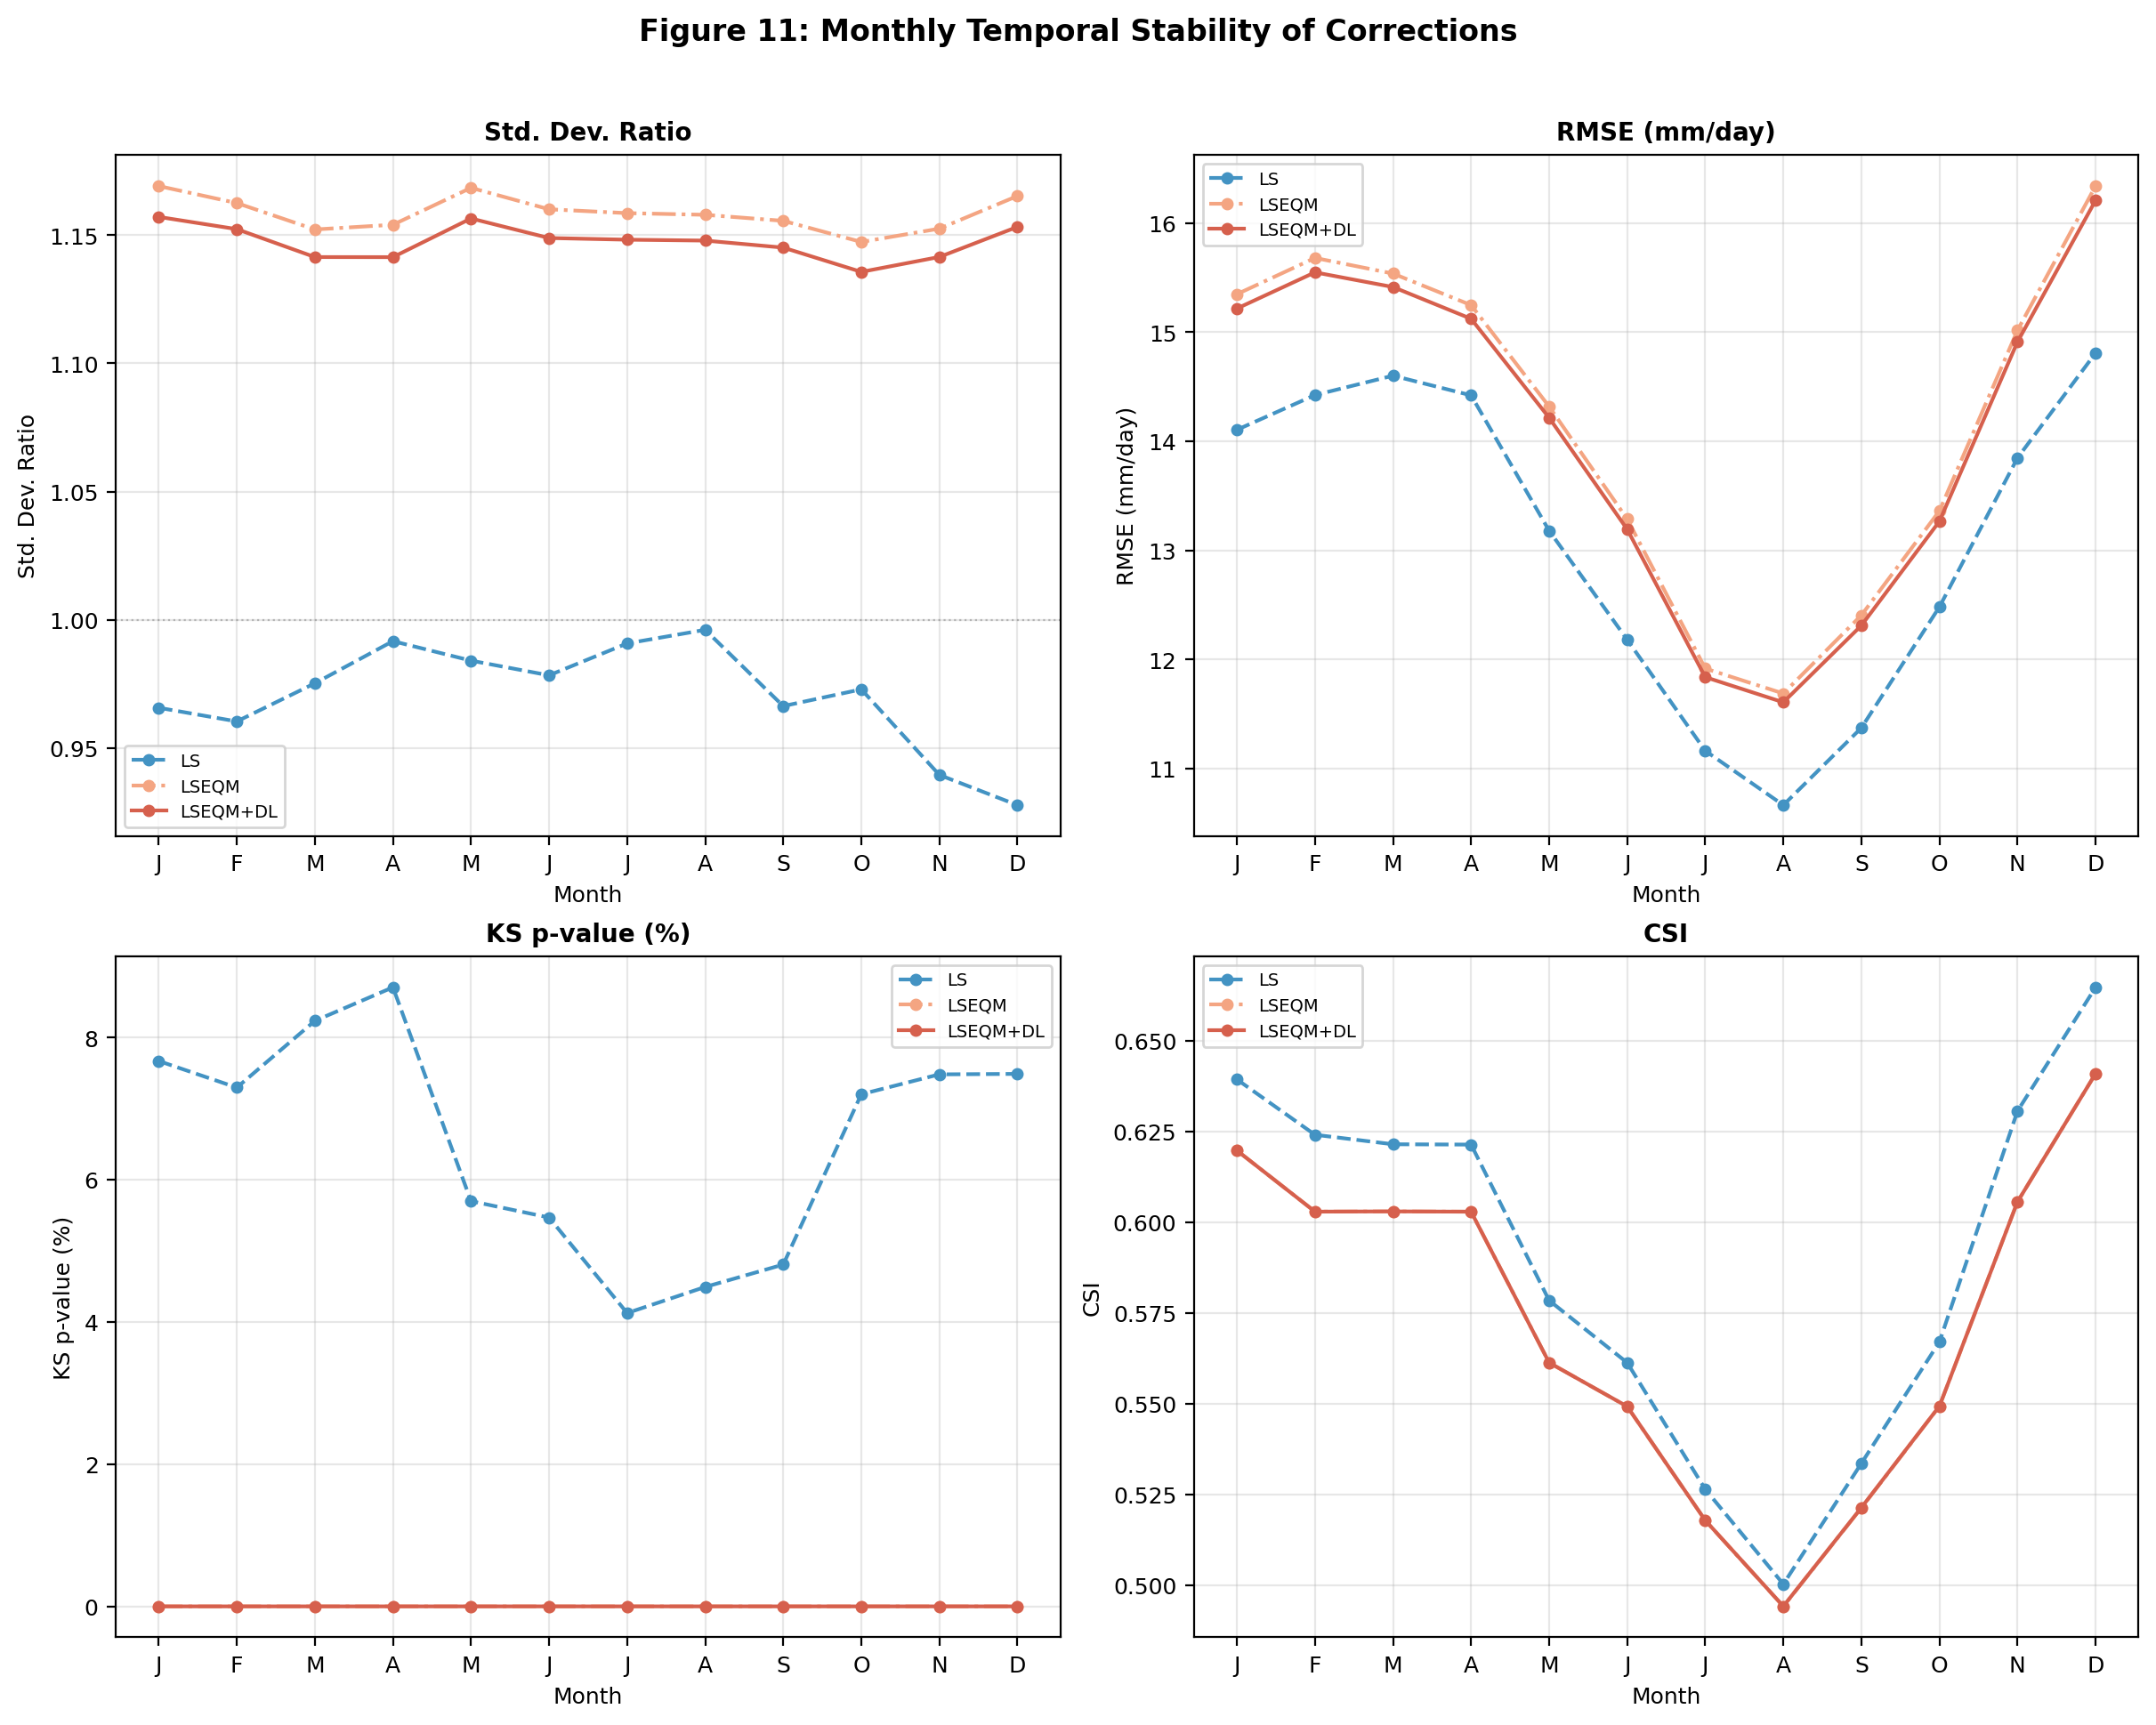
\includegraphics[width=\textwidth]{images/fig11_temporal_stability.png}
\caption{Monthly temporal stability of correction performance: (a) standard deviation ratio, (b) RMSE (mm/day), (c) KS \(p\)-value (\%), and (d) Critical Success Index (CSI). Lines show domain-median values for LS (blue), LSEQM (orange), and LSEQM+DL (green) across all 12 months. The seasonal cycle reflects the wet (October--March) and dry (April--September) monsoon regime.}\label{fig12}
\end{figure}

The relative ordering of correction methods is stable across all months: LSEQM and LSEQM+DL maintain consistently higher variability than LS (SDR 1.10--1.18 vs. 0.94--0.97), and the LS-to-LSEQM gap in CSI (\(\approx\) 0.02--0.03) is consistent across months. RMSE follows the expected seasonal pattern, peaking during the wet season. These results confirm that the distributional correction does not introduce seasonal artifacts and that the POD trade-off is not seasonally concentrated.

\subsection{Discussion}\label{discussion}

\paragraph{Synthesis}

The sequential design offers advantages over both purely statistical and purely DL approaches. Single-method statistical corrections can align distributions but may not capture complex spatial patterns \cite{ref8,ref44}. Standalone DL approaches risk introducing physically implausible values if inadequately constrained \cite{ref9,ref12}. By positioning the CNN as a refinement step after statistical correction, the DL component operates on partially corrected input from the same statistical domain used during training, avoiding the domain shift problem. The alpha-blending weight of 0.70 assigns dominant influence to the statistical correction, with CNN providing targeted refinement for extreme pixels only.

An important finding is that distributional bias correction does not improve, and is not designed to improve, temporal prediction skill at the pixel level \cite{ref34}. Applications requiring temporally accurate fields should use the corrected product in combination with temporal downscaling or ensemble methods. Additionally, IMERG-L is known to over-detect light precipitation over the Maritime Continent \cite{ref31,ref32}; this signature persists after LSEQM (\hyperref[progressive-improvement]{Section~3.1}, Supplementary~S4).

The station density confidence mask addresses a challenge common to all bias correction methods relying on gridded gauge products: spatial heterogeneity of reference quality. The mask adapts to whatever gauge network is available without manual tuning, scaling the CNN contribution with local reference reliability rather than applying or suppressing it uniformly. Within Indonesia, this design produces a within-domain gradient that doubles as a transferability indicator: in densely gauged Java the framework operates near its maximum capacity, while in sparsely gauged eastern Indonesia (Papua, Maluku, eastern Nusa Tenggara) it correctly reverts toward pure LSEQM. The performance metrics reported here therefore span both ends of the gauge-density spectrum the framework is designed to handle.

\subsubsection{Limitations}\label{limitations}

Several limitations should be acknowledged. The dekadal pooling strategy preserves seasonal characteristics but does not model temporal autocorrelation or inter-annual trends. The CPC-UNI reference at \(0.5^{\circ}\) is considerably coarser than the \(0.1^{\circ}\) IMERG grid; the BCSD strategy produces spatially smooth correction fields but does not introduce sub-grid variability in complex terrain. The CNN Flatten-Dense architecture was deliberately chosen as a lightweight refinement step; fully convolutional architectures (e.g., U-Net) could improve spatial fidelity \cite{ref40,ref41}.

The framework is demonstrated over a single domain (Indonesia, 2001--2025). While the methodology uses globally available datasets, the GPD threshold, CNN hyperparameters, and alpha-blending weight may require recalibration for different climate regimes \cite{ref44,ref45}. The evaluation uses the same temporal period for correction and assessment; a strict hold-out would strengthen generalization claims, though at the cost of reduced training samples. Independent BMKG station validation partially mitigates this concern.

The alpha-blending weight (\(\alpha = 0.70\)), GPD threshold percentile (80th), and station density saturation count (2 stations per \(0.5^{\circ}\) cell) were selected based on domain expertise rather than formal optimization. A sensitivity analysis could identify performance trade-offs and inform region-specific calibration. The CQI component weights represent a subjective but informed partitioning; the relative ranking of methods is expected to be robust to reasonable weight perturbations.

The performance numbers reported for eastern Indonesia represent a conservative case: the confidence mask correctly suppresses CNN influence where the reference is poorly constrained, so those metric values characterize the LSEQM stage operating with minimum gauge support, not the full hybrid framework. Applications in regions with denser networks than the CPC-UNI input (180 stations for Indonesia) would admit higher CNN influence than the \(\alpha = 0.70\) cap allows here. This is a property of the design, not a recalibration claim: the numerical values for the GPD threshold, alpha, and saturation count remain region-specific, but the framework's graceful degradation under sparse data is general.

\paragraph{Residual Bias Attribution}\label{residual-bias-attribution}

After LSEQM correction, a residual positive bias of approximately \(+8\%\) against CPC-UNI persists during peak monsoon, reduced from \(+15.5\%\) for the raw product. This residual is structural rather than methodological, arising from two factors: CPC-UNI systematically undercatches convective precipitation over sparsely gauged terrain \cite{ref36,ref37}, and the \(0.5^{\circ}\) gauge analysis cannot resolve sub-grid heterogeneity present in the \(0.1^{\circ}\) satellite retrieval. The \(+8\%\) residual falls at the lower end of published IMERG-L wet-season biases over the Maritime Continent (\(+10\%\) to \(+25\%\)) \cite{ref31,ref32,ref33,ref38,ref39,ref47}.

The conditional bias decomposition (Supplementary S4) confirms that this residual reflects a mismatch in \emph{which days are heavy where} between IMERG and the gauge analysis, a conditional error that cannot be removed by univariate quantile mapping by construction \cite{ref34,ref11}. Station-level validation (\hyperref[station-level-ground-truth-validation]{Section~3.5}) shows that LSEQM moves the standard deviation ratio, wet-day frequency, and \(Q_{99}\) toward gauge observations even where it moves away from CPC-UNI, consistent with reference-side undercatch as the dominant explanation. Partial contributions from GPD parameter uncertainty cannot be ruled out without a formal sensitivity analysis of fitted shape and scale parameters; the consistent direction of LSEQM-vs-station agreement (SDR, KS \(p\), and \(Q_{99}\) all moving toward target) places an upper bound on the magnitude of any correction-side over-shoot.

\subsubsection{Future Directions}\label{future-directions}

Several extensions merit investigation: (1) replacing the Dense reconstruction with a fully convolutional architecture (e.g., U-Net) and incorporating auxiliary features (elevation, land cover) as CNN input channels; (2) extending to other satellite products (CHIRPS, GSMaP, MSWEP \cite{ref42}) and other tropical regions (Sub-Saharan Africa, Amazon basin) to test transferability; (3) refining the temporal scale from dekadal to pentad or daily corrections with adaptive window sizing; and (4) conducting formal sensitivity analysis of the alpha-blending weight and GPD threshold using cross-validated grid search \cite{ref43}, alongside a strict temporal hold-out experiment.

\section{Conclusions}\label{conclusions}

This study developed and evaluated a modular hybrid bias correction
framework (LSEQM+DL) for daily satellite precipitation, integrating
Linear Scaling, Empirical Quantile Mapping with GPD tail adjustment,
and CNN refinement modulated by a station density confidence mask.
Applied to IMERG Late Run over Indonesia (2001--2025) and evaluated
against CPC-UNI and 171 BMKG station observations, the framework
delivers measurable improvements across the three design objectives:
adjusting values, aligning distributions, and preserving extremes.

At independent BMKG stations, the standard deviation ratio moves from
0.71 (LS) to 1.00 (LSEQM+DL), the wet-day frequency bias decreases from
21\% to 5\%, the \(Q_{99}\) ratio improves from 0.71 to 1.01, and the
relative bias contracts from \(-\)11.4\% to \(-\)0.6\%. These improvements
come at a measurable cost in event detection (POD: 0.78 to 0.65), a
trade-off inherent to the dry-day frequency matching \cite{ref11} that
is partially offset by improved FAR (0.36 to 0.32). At thresholds above
20~mm/day, LSEQM+DL maintains higher detection skill than LS (CSI at
50~mm improves from 0.062 to 0.097); statistical significance of these
threshold-by-threshold differences was not formally tested.

Pixel-level temporal accuracy (correlation, RMSE, NSE) remains largely
unchanged across correction stages, consistent with the theoretical
expectation that quantile mapping adjusts marginal distributions without
modifying temporal sequencing \cite{ref34}. The corrected product
therefore offers improved statistical properties (bias, variability,
distribution shape, extreme magnitudes) but not improved day-to-day
prediction accuracy. The station density confidence mask provides
graceful degradation in data-sparse regions, allowing CNN refinement
where the reference is well constrained while reverting to pure LSEQM
elsewhere; the mask also serves as a spatially explicit quality flag.

Several limitations warrant consideration: the absence of a strict
temporal hold-out, the use of a relatively simple CNN architecture
trained per-dekad on \(\sim\)230 daily fields, and the reliance on
fixed values for the blending weight, GPD threshold, and saturation
count that were not formally optimized. The framework relies on globally
available datasets (IMERG and CPC-UNI) and is portable in principle to
other tropical regions with regional recalibration of these parameters.
Future work targets formal sensitivity analysis, alternative
architectures such as U-Net, and transfer to additional Maritime
Continent and other tropical domains.

%%%%%%%%%%%%%%%%%%%%%%%%%%%%%%%%%%%%%%%%%%


\begin{thebibliography}{47}


\bibitem{ref1} Hou, A.Y., Kakar, R.K., Neeck, S., Azarbarzin, A.A., Kummerow,
C.D., Kojima, M., Oki, R., Nakamura, K. and Iguchi, T. (2014). The
Global Precipitation Measurement Mission. \emph{Bull. Amer. Meteor.
Soc.}, 95(5), 701-722. DOI: 10.1175/BAMS-D-13-00164.1

\bibitem{ref2} Huffman, G.J., Bolvin, D.T., Braithwaite, D., Hsu, K.-L., Joyce,
R.J., Kidd, C., Nelkin, E.J., Sorooshian, S., Stocker, E.F., Tan, J.,
Wolff, D.B. and Xie, P. (2020). Integrated Multi-satellitE Retrievals
for the Global Precipitation Measurement (GPM) Mission (IMERG).
\emph{Satellite Precipitation Measurement}, Adv. Global Change Res., 67,
343-353. DOI: 10.1007/978-3-030-24568-9\_19

\bibitem{ref3} Maggioni, V., Meyers, P.C. and Robinson, M.D.~(2016). A Review
of Merged High-Resolution Satellite Precipitation Product Accuracy
during the Tropical Rainfall Measuring Mission (TRMM) Era. \emph{J.
Hydrometeor.}, 17(4), 1101-1117. DOI: 10.1175/JHM-D-15-0190.1

\bibitem{ref4} Teutschbein, C. and Seibert, J. (2012). Bias correction of
regional climate model simulations for hydrological climate-change
impact studies: Review and evaluation of different methods. \emph{J.
Hydrol.}, 456-457, 12-29. DOI: 10.1016/j.jhydrol.2012.05.052

\bibitem{ref5} Gudmundsson, L., Bremnes, J.B., Haugen, J.E. and Engen-Skaugen,
T. (2012). Technical Note: Downscaling RCM precipitation to the station
scale using statistical transformations -- a comparison of methods.
\emph{Hydrol. Earth Syst. Sci.}, 16, 3383-3390. DOI:
10.5194/hess-16-3383-2012

\bibitem{ref6} Themessl, M.J., Gobiet, A. and Heinrich, G. (2012).
Empirical-statistical downscaling and error correction of regional
climate models and its impact on the climate change signal.
\emph{Climatic Change}, 112, 449-468. DOI: 10.1007/s10584-011-0224-4

\bibitem{ref7} Coles, S. (2001). \emph{An Introduction to Statistical Modeling
of Extreme Values}. Springer Series in Statistics. DOI:
10.1007/978-1-4471-3675-0

\bibitem{ref8} Maraun, D. (2016). Bias Correcting Climate Change Simulations --
a Critical Review. \emph{Curr. Clim. Change Rep.}, 2, 211-220. DOI:
10.1007/s40641-016-0050-x

\bibitem{ref9} Bano-Medina, J., Manzanas, R. and Gutierrez, J.M. (2020).
Configuration and intercomparison of deep learning neural models for
statistical downscaling. \emph{Geosci. Model Dev.}, 13, 2109-2124. DOI:
10.5194/gmd-13-2109-2020

\bibitem{ref10} Pan, B., Hsu, K., AghaKouchak, A. and Sorooshian, S. (2019).
Improving Precipitation Estimation Using Convolutional Neural Network.
\emph{Water Resour. Res.}, 55(3), 2301-2321. DOI: 10.1029/2018WR024090

\bibitem{ref11} Cannon, A.J., Sobie, S.R. and Murdock, T.Q. (2015). Bias
Correction of GCM Precipitation by Quantile Mapping: How Well Do Methods
Preserve Changes in Quantiles and Extremes? \emph{J. Climate}, 28(17),
6938-6959. DOI: 10.1175/JCLI-D-14-00754.1

\bibitem{ref12} Ehret, U., Zehe, E., Wulfmeyer, V., Warrach-Sagi, K. and
Liebert, J. (2012). HESS Opinions: Should we apply bias correction to
global and regional climate model data? \emph{Hydrol. Earth Syst. Sci.},
16, 3391-3404. DOI: 10.5194/hess-16-3391-2012

\bibitem{ref13} Chen, M., Shi, W., Xie, P., Silva, V.B.S., Kousky, V.E., Wayne
Higgins, R. and Janowiak, J.E. (2008). Assessing objective techniques
for gauge-based analyses of global daily precipitation. \emph{J.
Geophys. Res.}, 113, D04110. DOI: 10.1029/2007JD009132

\bibitem{ref14} Ebert, E.E. (2007). Methods for Verifying Satellite
Precipitation Estimates. \emph{Measuring Precipitation from Space}, Adv.
Global Change Res., 28, 345-356. DOI: 10.1007/978-1-4020-5835-6\_27

\bibitem{ref15} Wilks, D.S. (2011). \emph{Statistical Methods in the
Atmospheric Sciences}. 3rd ed.~Academic Press, International Geophysics
Series, Vol. 100. DOI: 10.1016/B978-0-12-385022-5.00001-4

\bibitem{ref16} Piani, C., Haerter, J.O. and Coppola, E. (2010). Statistical
bias correction for daily precipitation in regional climate models over
Europe. \emph{Theor. Appl. Climatol.}, 99, 187-192. DOI:
10.1007/s00704-009-0134-9

\bibitem{ref17} LeCun, Y., Bengio, Y. and Hinton, G. (2015). Deep learning.
\emph{Nature}, 521, 436-444. DOI: 10.1038/nature14539

\bibitem{ref18} Xie, P., Chen, M., Yang, S., Yatagai, A., Hayasaka, T.,
Fukushima, Y. and Liu, C. (2007). A Gauge-Based Analysis of Daily
Precipitation over East Asia. \emph{J. Hydrometeor.}, 8(3), 607-626.
DOI: 10.1175/JHM583.1

\bibitem{ref19} Aldrian, E. and Susanto, R.D. (2003). Identification of three
dominant rainfall regions within Indonesia and their relationship to sea
surface temperature. \emph{Int. J. Climatol.}, 23(12), 1435-1452. DOI:
10.1002/joc.950

\bibitem{ref20} As-syakur, A.R., Tanaka, T., Osawa, T. and Mahendra, M.S.
(2013). Indonesian rainfall variability observation using TRMM
multi-satellite data. \emph{Int. J. Remote Sens.}, 34(21), 7723-7738.
DOI: 10.1080/01431161.2013.826837

\bibitem{ref21} Pradhan, R.K., Markonis, Y., Varber, M.R., Franch, M.,
Papalexiou, S.M., Vidal, J.-P., Pappas, C., Hanel, M. and Hao, Z.
(2022). Review of GPM IMERG performance: A global perspective.
\emph{Remote Sens. Environ.}, 268, 112754. DOI:
10.1016/j.rse.2021.112754

\bibitem{ref22} Sun, Q., Miao, C., Duan, Q., Ashouri, H., Sorooshian, S. and
Hsu, K.-L. (2018). A Review of Global Precipitation Data Sets: Data
Sources, Estimation, and Intercomparisons. \emph{Rev.~Geophys.}, 56(1),
79-107. DOI: 10.1002/2017RG000574

\bibitem{ref23} Wood, A.W., Leung, L.R., Sridhar, V. and Lettenmaier, D.P.
(2004). Hydrologic implications of dynamical and statistical approaches
to downscaling climate model outputs. \emph{Climatic Change}, 62,
189-216. DOI: 10.1023/B:CLIM.0000013685.99609.9e

\bibitem{ref24} WMO (2008). \emph{Guide to Meteorological Instruments and
Methods of Observation}. WMO-No.~8, World Meteorological Organization,
Geneva.

\bibitem{ref25} Hosking, J.R.M. and Wallis, J.R. (1997). \emph{Regional
Frequency Analysis: An Approach Based on L-Moments}. Cambridge
University Press. DOI: 10.1017/CBO9780511529443

\bibitem{ref26} Kingma, D.P. and Ba, J. (2015). Adam: A Method for Stochastic
Optimization. \emph{Proc. 3rd Int. Conf. Learning Representations (ICLR
2015)}, San Diego.

\bibitem{ref27} Mega, T., Ushio, T., Matsuda, T., Kubota, T., Kachi, M. and
Oki, R. (2019). Gauge-Adjusted Global Satellite Mapping of
Precipitation. \emph{IEEE Trans. Geosci. Remote Sens.}, 57(4),
1928-1935. DOI: 10.1109/TGRS.2018.2870199

\bibitem{ref28} Nash, J.E. and Sutcliffe, J.V. (1970). River flow forecasting
through conceptual models part I -- A discussion of principles. \emph{J.
Hydrol.}, 10(3), 282-290. DOI: 10.1016/0022-1694(70)90255-6

\bibitem{ref29} Moriasi, D.N., Arnold, J.G., Van Liew, M.W., Bingner, R.L.,
Harmel, R.D. and Veith, T.L. (2007). Model evaluation guidelines for
systematic quantification of accuracy in watershed simulations.
\emph{Trans. ASABE}, 50(3), 885-900. DOI: 10.13031/2013.23153

\bibitem{ref30} Gupta, H.V., Kling, H., Yilmaz, K.K. and Martinez, G.F. (2009).
Decomposition of the mean squared error and NSE performance criteria:
Implications for improving hydrological modelling. \emph{J. Hydrol.},
377(1-2), 80-91. DOI: 10.1016/j.jhydrol.2009.08.003

\bibitem{ref31} Tan, J., Petersen, W.A. and Tokay, A. (2016). A Novel Approach
to Identify Sources of Errors in IMERG for GPM Ground Validation.
\emph{J. Hydrometeor.}, 17(9), 2477-2491. DOI: 10.1175/JHM-D-16-0079.1

\bibitem{ref32} Ramadhan, R., Yusnaini, H., Marzuki, M., Muharsyah, R., Suryanto, W., Sholihun, S., Vonnisa, M., Harmadi, H., Ningsih, A.P., Battaglia, A., Hashiguchi, H. and Tokay, A. (2022). Evaluation of GPM IMERG Performance Using Gauge Data over Indonesian Maritime Continent at Different Time Scales.
\emph{Remote Sensing}, 14(5), 1172. DOI: 10.3390/rs14051172

\bibitem{ref33} Tang, G., Clark, M.P., Papalexiou, S.M., Ma, Z. and Hong, Y.
(2020). Have satellite precipitation products improved over last two
decades? A comprehensive comparison of GPM IMERG with nine satellite and
reanalysis datasets. \emph{Remote Sens. Environ.}, 240, 111697. DOI:
10.1016/j.rse.2020.111697

\bibitem{ref34} Maraun, D. (2013). Bias correction, quantile mapping, and
downscaling: Revisiting the inflation issue. \emph{J. Climate}, 26(6),
2137-2143. DOI: 10.1175/JCLI-D-12-00821.1

\bibitem{ref35} Taylor, K.E. (2001). Summarizing multiple aspects of model
performance in a single diagram. \emph{J. Geophys. Res.}, 106(D7),
7183-7192. DOI: 10.1029/2000JD900719

\bibitem{ref36} Adam, J.C. and Lettenmaier, D.P. (2003). Adjustment of global
gridded precipitation for systematic bias. \emph{J. Geophys. Res.},
108(D9), 4257. DOI: 10.1029/2002JD002499

\bibitem{ref37} Behrangi, A., Khakbaz, B., Jaw, T.C., AghaKouchak, A., Hsu, K.
and Sorooshian, S. (2011). Hydrologic evaluation of satellite
precipitation products over a mid-size basin. \emph{J. Hydrol.},
397(3-4), 225-237. DOI: 10.1016/j.jhydrol.2010.11.043

\bibitem{ref38} Rahmawati, N. and Lubczynski, M.W. (2018). Validation of
satellite daily rainfall estimates in complex terrain of Bali Island,
Indonesia. \emph{Theor. Appl. Climatol.}, 134(1--2), 513--532. DOI:
10.1007/s00704-017-2290-7

\bibitem{ref39} Wang, Z., Zhong, R., Lai, C. and Chen, J. (2017). Evaluation of
the GPM IMERG satellite-based precipitation products and the
hydrological utility. \emph{Atmos. Res.}, 196, 151-163. DOI:
10.1016/j.atmosres.2017.06.020

\bibitem{ref40} Sha, Y., Gagne II, D.J., West, G. and Stull, R. (2020).
Deep-learning-based gridded downscaling of surface meteorological
variables in complex terrain. Part I: Daily maximum and minimum 2-m
temperature. \emph{J. Appl. Meteor. Climatol.}, 59(12), 2057-2073. DOI:
10.1175/JAMC-D-20-0057.1

\bibitem{ref41} Vandal, T., Kodra, E., Ganguly, S., Michaelis, A., Nemani, R.
and Ganguly, A.R. (2017). DeepSD: Generating high fidelity daily climate
surfaces with generative adversarial networks. \emph{Proc. 23rd ACM
SIGKDD Int. Conf. on Knowledge Discovery and Data Mining}, 1375-1383.
DOI: 10.1145/3097983.3098004

\bibitem{ref42} Beck, H.E., Wood, E.F., Pan, M., Fisher, C.K., Miralles, D.G.,
van Dijk, A.I.J.M., McVicar, T.R. and Adler, R.F. (2019). MSWEP V2
Global 3-Hourly 0.1 degrees Precipitation: Methodology and Quantitative
Assessment. \emph{Bull. Amer. Meteor. Soc.}, 100(3), 473-500. DOI:
10.1175/BAMS-D-17-0138.1

\bibitem{ref43} Lange, S. (2019). Trend-preserving bias adjustment and
statistical downscaling with ISIMIP3BASD (v1.0). \emph{Geosci. Model
Dev.}, 12, 3055-3070. DOI: 10.5194/gmd-12-3055-2019

\bibitem{ref44} Hempel, S., Frieler, K., Warszawski, L., Schewe, J. and
Piontek, F. (2013). A trend-preserving bias correction -- the ISI-MIP
approach. \emph{Earth Syst. Dynam.}, 4, 219-236. DOI:
10.5194/esd-4-219-2013

\bibitem{ref45} Baez-Villanueva, O.M., Zambrano-Bigiarini, M., Beck, H.E.,
McNamara, I., Ribbe, L., Nauditt, A., Birkel, C., Verbist, K.,
Giraldo-Osorio, J.D. and Thinh, N.X. (2020). RF-MEP: A novel Random
Forest method for merging gridded precipitation products and
ground-based measurements. \emph{Remote Sens. Environ.}, 239, 111606.
DOI: 10.1016/j.rse.2019.111606

\bibitem{ref46} Sillmann, J., Kharin, V.V., Zhang, X., Zwiers, F.W. and
Bronaugh, D. (2013). Climate extremes indices in the CMIP5 multimodel
ensemble: Part 1. Model evaluation in the present climate. \emph{J.
Geophys. Res. Atmos.}, 118, 1716-1733. DOI: 10.1002/jgrd.50203

\bibitem{ref47} Wu, P., Yamanaka, M.D.~and Matsumoto, J. (2008). The Formation
of Nocturnal Rainfall Offshore from Convection over Western Kalimantan
(Borneo) Island. \emph{J. Meteor. Soc. Japan}, 86A, 187-203. DOI:
10.2151/jmsj.86A.187


\end{thebibliography}

\end{document}
